% 施工稿：复制自 paper02_CN.tex，2026-09-29，PaperRefinePrompt v3
%%
%% The original source files were:
%%
%% samples.dtx  (with options: `all,proceedings,bibtex,manuscript')
%% 
%% IMPORTANT NOTICE:
%% 
%% For the copyright see the source file.
%% 
%% Any modified versions of this file must be renamed
%% with new filenames distinct from sample-manuscript.tex.
%% 
%% For distribution of the original source see the terms
%% for copying and modification in the file samples.dtx.
%% 
%% This generated file may be distributed as long as the
%% original source files, as listed above, are part of the
%% same distribution. (The sources need not necessarily be
%% in the same archive or directory.)
%%
%%
%% Commands for TeXCount
%TC:macro \cite [option:text,text]
%TC:macro \citep [option:text,text]
%TC:macro \citet [option:text,text]
%TC:envir table 0 1
%TC:envir table* 0 1
%TC:envir tabular [ignore] word
%TC:envir displaymath 0 word
%TC:envir math 0 word
%TC:envir comment 0 0
%%
%% The first command in your LaTeX source must be the \documentclass
%% command.
%%
%% For submission and review of your manuscript please change the
%% command to \documentclass[manuscript, screen, review]{acmart}.
%%
%% When submitting camera ready or to TAPS, please change the command
%% to \documentclass[sigconf]{acmart} or whichever template is required
%% for your publication.
%%
%%
\documentclass[manuscript,screen,review]{acmart}


\usepackage{algorithm}
% Use algorithmicx + algpseudocode: provides \Require, \Ensure, \State, and \Comment
\usepackage{algorithmicx}
\usepackage{algpseudocode}
% Provide compatibility shims for uppercase macros used in the document
% Some authors use \REQUIRE/\ENSURE/\UPON/\ENDUPON (uppercase) — map them to algpseudocode
\providecommand{\REQUIRE}[1]{\Require{#1}}
\providecommand{\ENSURE}[1]{\Ensure{#1}}
% \UPON{<cond>} will render as a bold 'Upon <cond>' state line inside algorithmic blocks
\providecommand{\UPON}[1]{\State\textbf{Upon}~#1}
\providecommand{\ENDUPON}{}
% Provide uppercase aliases commonly used in algorithm blocks
\providecommand{\STATE}{\State}
\providecommand{\COMMENT}[1]{\Comment{#1}}
% Map common uppercase algorithmic keywords to algorithmicx/algpseudocode commands
\providecommand{\IF}{\If}
\providecommand{\ELSE}{\Else}
\providecommand{\ELSIF}{\ElsIf}
\providecommand{\ENDIF}{\EndIf}
\providecommand{\FOR}{\For}
\providecommand{\ENDFOR}{\EndFor}
\providecommand{\WHILE}{\While}
\providecommand{\ENDWHILE}{\EndWhile}
\providecommand{\RETURN}{\State\textbf{return}~}
% color support for \textcolor used inside algorithms
\usepackage{xcolor}
% Math packages required for \text and bold symbols inside math
\usepackage{amsmath}
\usepackage{bm}
% Define common math operators used in the document
\DeclareMathOperator*{\argmin}{arg\,min}
\DeclareMathOperator*{\argmax}{arg\,max}
\usepackage{multirow}
% Enable list customization (leftmargin, itemsep, etc.) used in the document
\usepackage{enumitem}
% Ensure header height is sufficient for fancyhdr
\setlength{\headheight}{20.48303pt}
% theorem environments used in the document
% acmart/amsart already provides amsthm; do not load amsthm again
\newtheorem{assumption}{假设}
\newtheorem{problem}{问题}
\renewcommand{\proofname}{证明}
\AtEndPreamble{%
  \let\proposition\relax
  \let\endproposition\relax
  \newtheorem{proposition}[theorem]{命题}%
}
% 中文初稿：请用 XeLaTeX 编译
\usepackage{xeCJK}
\setCJKmainfont{SimSun}[BoldFont=SimHei]
\setCJKsansfont{SimHei}
\xeCJKsetup{PunctStyle=kaiming}

%%
%% \BibTeX command to typeset BibTeX logo in the docs
\AtBeginDocument{%
  \providecommand\BibTeX{{%
    Bib\TeX}}}

%% Rights management information.  This information is sent to you
%% when you complete the rights form.  These commands have SAMPLE
%% values in them; it is your responsibility as an author to replace
%% the commands and values with those provided to you when you
%% complete the rights form.
\setcopyright{acmlicensed}
\copyrightyear{2026}
\acmYear{2026}
\acmDOI{XXXXXXX.XXXXXXX}

%% These commands are for a PROCEEDINGS abstract or paper.
%%  \acmConference[Conference acronym 'XX]{Make sure to enter the correct
%% 	conference title from your rights confirmation email}{June 03--05,
%% 	2018}{Woodstock, NY}

%%
%%  Uncomment \acmBooktitle if the title of the proceedings is different
%%  from ``Proceedings of ...''!
%%
%%\acmBooktitle{Woodstock '18: ACM Symposium on Neural Gaze Detection,
%%  June 03--05, 2018, Woodstock, NY}
%%\acmISBN{978-1-4503-XXXX-X/2018/06}


%%
%% Submission ID.
%% Use this when submitting an article to a sponsored event. You'll
%% receive a unique submission ID from the organizers
%% of the event, and this ID should be used as the parameter to this command.
%%\acmSubmissionID{123-A56-BU3}

%%
%% For managing citations, it is recommended to use bibliography
%% files in BibTeX format.
%%
%% You can then either use BibTeX with the ACM-Reference-Format style,
%% or BibLaTeX with the acmnumeric or acmauthoryear sytles, that include
%% support for advanced citation of software artefact from the
%% biblatex-software package, also separately available on CTAN.
%%
%% Look at the sample-*-biblatex.tex files for templates showcasing
%% the biblatex styles.
%%

%%
%% The majority of ACM publications use numbered citations and
%% references.  The command \citestyle{authoryear} switches to the
%% "author year" style.
%%
%% If you are preparing content for an event
%% sponsored by ACM SIGGRAPH, you must use the "author year" style of
%% citations and references.
%% Uncommenting
%% the next command will enable that style.
%%\citestyle{acmauthoryear}


%%
%% end of the preamble, start of the body of the document source.
\begin{document}

%%
%% The "title" command has an optional parameter,
%% allowing the author to define a "short title" to be used in page headers.
\title[离散事件注入攻击检测]{基于硬约束层与半马尔可夫时序通道的工业离散事件注入检测}
\subtitle{Reference-Model Hard Constraints and Semi-Markov Timing Channels for Detecting Injection Attacks on Discrete Industrial Event Streams}

%%
%% The "author" command and its associated commands are used to define
%% the authors and their affiliations.
%% Of note is the shared affiliation of the first two authors, and the
%% "authornote" and "authornotemark" commands
%% used to denote shared contribution to the research.
\author{Qi Yu}
%%\authornote{.}
%%\authornotemark[1]
\email{230240012@seu.edu.cn}
%%\orcid{1234-5678-9012}
\affiliation{%
	\institution{School of Cyber Science and Engineering, Southeast University}
	\city{Nanjing}
	\state{Jiangsu}
	\country{PR China}
}


\author{Wei Li}
%%\orcid{1234-5678-9012}
\email{xchlw@seu.edu.cn}
\authornote{corresponding author}
%%\authornotemark[1]
\affiliation{%
	\institution{School of Computer Science and Engineering, Southeast University}
	\city{Nanjing}
	\state{Jiangsu}
	\country{PR China}
}


%%
%% By default, the full list of authors will be used in the page
%% headers. Often, this list is too long, and will overlap
%% other information printed in the page headers. This command allows
%% the author to define a more concise list
%% of authors' names for this purpose.
%%\renewcommand{\shortauthors}{Qi et al.}

%%
%% The abstract is a short summary of the work to be presented in the
%% article.
\begin{abstract}
工业信息物理生产系统中，现场设备以带生命周期（指派、开始、完成）的离散活动事件上报运行过程，攻击者在上行链路上注入或重放这些事件，即可使日志与物理过程脱节。仅依据标签预测概率设定阈值的检测方法对此存在结构性盲区：在零误报约束下，它只能标记工艺参考模型本就禁止的转移；对不改动标签、只压缩停留时长的伪造，其净检出为零。
本文构建三路并行检测：硬约束层以参考模型导出的可行性掩码直接否决不可行事件；半马尔可夫时序通道以分组对数正态停留时长给出残差；结构通道度量作业实例内的活动转移是否罕见。两路统计通道经共形预测校准后，由累积和（CUSUM）检验逐条累积证据，误报预算在三路之间均分。理论上，本文以命题刻画仅标签检测族的盲区，并给出临界相对提前量 $\rho^*(\alpha,\sigma)$，即单条伪造被检出概率达到一半时的停留缩短比例。
本文在 Fischertechnik Trier 真实产线日志上按可复现协议合成六类攻击。在误报预算 $\alpha=0.01$、延迟预算 $10$ 条、扣除偶然告警基线的口径下，本文对物理不可行注入的净检出为 $0.95$；对渐变漂移为 $0.87$，而仅标签消融为 $0$；对提前完成重放（注入率 $20\%$）为 $0.18$，高于计时自动机基线（配对检验显著），与计时自动机结合贝叶斯网络的基线差异不显著。
状态模仿与消息抑制上，本文低于仅标签消融。结论基于单一公开日志与合成注入；门限改在校准折标定时，各方法误报均超出名义值。
\end{abstract}

\begin{CCSXML}
<ccs2012>
   <concept>
       <concept_id>10002978.10003006.10003013</concept_id>
       <concept_desc>Security and privacy~Intrusion detection systems</concept_desc>
       <concept_significance>500</concept_significance>
       </concept>
   <concept>
       <concept_id>10010520.10010521</concept_id>
       <concept_desc>Computer systems organization~Embedded and cyber-physical systems</concept_desc>
       <concept_significance>300</concept_significance>
       </concept>
</ccs2012>
\end{CCSXML}

\ccsdesc[500]{Security and privacy~Intrusion detection systems}
\ccsdesc[300]{Computer systems organization~Embedded and cyber-physical systems}

\begin{keywords}
注入攻击检测, 离散事件日志, 半马尔可夫过程, 可行性掩码,
共形预测, 序贯检验, 信息物理生产系统
\end{keywords}

\maketitle


%=============================================================================
\section{引言}
\label{sec:intro}

\subsection{研究背景与动机}
\label{sec:intro_bg}

信息物理生产系统（cyber-physical production system, CPPS）中，现场设备以离散活动事件上报运行过程：一条事件包含设备、操作（或状态标签）、时间戳与作业实例~\cite{monostori2016cpps,seiger2022factory}。例如，调度系统向搬运设备下达``前往某工位''的指派后，日志依次记录指派、开始执行与完成，每项活动因此具有从指派到完成的生命周期。攻击者无须改写连续控制律或攻破设备固件，只需在上行链路上\textbf{注入或重放这些事件}，即可使日志记录的轨迹与物理过程脱节。工业信息物理系统上的检测文献主要集中于过程物理量、边界防护与网络流量~\cite{kayan2022icps}，带生命周期的活动事件很少被单独视为注入对象。本文检测的是这些事件是否被注入或重放，不评测调度器据此如何派工。

典型的攻击手法是在活动尚未完成时重放``已完成''事件。单条记录在标签层面完全合法，却改写了停留时长与后继事件的上下文。仅比较预测标签与观测标签的检测器无法识别此类注入：其判决只取决于（前驱，标签）这一对取值，与该条记录是良性还是伪造无关，见命题~\ref{prop:ta}。

另一方面，同一条事件流同时具备三类可供检测器利用的结构，分别对应不同类型的注入。第一是可行性：工艺流程规定了哪台设备允许执行哪个操作、可由哪个前驱操作到达。这些约束由参考过程模型给出，无法从运行日志中学习得到，因为日志只记录历史上出现过的组合，无法区分``未曾观测''与``不允许''。第二是时长：活动消耗物理时间，标签序列合法但耗时错位的事件，在纯标签模型下与正常事件无从区分，只能依靠停留时长识别。第三是工作流结构：同一作业实例内活动的转移频率，插入或删除活动会改变转移序列。此外，完成事件与日志中指派的因果配对可作为硬约束层的附加检查。

\subsection{与已有工作的差距}
\label{sec:intro_gap}

既有检测工作未利用上述结构，原因在其方法论前提。面向产线的计时自动机~\cite{maier2011timed}为控制状态空间规模，将系统拆分为各自独立建模的组件，跨组件的可行性约束因此无法表达。TABOR~\cite{lin2018tabor}将计时自动机与贝叶斯网络结合，但依赖关系限制在同一工段之内，且不使用指派（命令）数据。确定性计数计时自动机 DCTA~\cite{barsha2024dcta}约束的是智能电网 {SCADA} 的通信协议会话，与工艺流程无关。连续控制层上的抗注入与抗重放研究~\cite{elsisi2023agv,mo2009replay}处理的是位置、速度等连续状态估计，而非离散活动事件。详细比较见第~\ref{sec:related}~节。

\subsection{本文方法}
\label{sec:intro_method}

本文以三路并行通道分别利用上述三类结构。硬约束层以参考模型导出的可行性掩码直接否决不可行事件，并附带检查指派--完成配对；时序通道按（设备，操作）分组，以对数正态停留时长给出标准化残差；结构通道以作业实例内工作流的转移概率度量活动是否罕见。两路统计通道经共形预测校准后，由 {CUSUM} 检验逐条累积证据。

时序建模本身并非新意：计时自动机已用于生产线与 {SCADA} 的时序异常检测~\cite{maier2011timed,lin2018timing}，隐半马尔可夫模型对停留时长的建模亦属成熟做法~\cite{tan2008hsmm}。本文与这些工作的差别在两处。其一，计时自动机的时钟守卫是区间型二值判断，落在区间之内的小幅提前上报会被直接接受；分布型停留时长则把这类同向偏差转化为可累积的证据。其二，数据驱动模型会把训练数据中未出现的活动组合判为异常，从而把新产品变体误判为攻击；参考模型可行性只拒绝工艺上不允许的组合。

\subsection{主要结果}
\label{sec:intro_results}

实验采用误报预算 $\alpha=0.01$ 与 $10$ 条消息的延迟预算（注入后 $10$ 条消息之内出现告警即判为检出），报告的净检出率已扣除窗口内随机误报造成的偶然告警基线。六类攻击依次为朴素重放（{A1}）、物理不可行注入（{A2}）、提前完成重放（{A3}）、状态模仿（{A4}）、渐变漂移（{A5}）与消息抑制（{A6}），定义见第~\ref{sec:coverage}~节。主要结果如下：{A2} 由参考模型规定的设备能力集覆盖，净检出 $0.95$；{A5} 上本文为 $0.87$，去掉时间维度的仅标签消融为 $0.00$；{A3} 上（注入率 $20\%$）本文为 $0.18{\pm}0.01$，高于 {BUTLA} 的 $0.10$（配对检验，{Holm} $p=0.031$），与 {TABOR} 式基线的差异校正后不显著（$p=0.096$），注入率降至 $10\%$ 及以下时不再占优；{A4}/{A6} 上本文低于仅标签消融（原因见第~\ref{sec:limitations}~节）。门限改在校准折标定时，各方法误报均超出名义值（本文 $0.030$）。按工序混合的临界相对提前量模型所预测的单消息功效曲线与实测吻合，平均绝对偏差约为 $0.03$。详见第~\ref{sec:experiments}~节。

\subsection{贡献}
\label{sec:intro_contrib}

本文的贡献如下。
\begin{enumerate}
\item \textbf{形式化带生命周期的离散活动事件上的注入检测问题。}
检测对象是带生命周期的活动事件（指派、开始、完成），既不是连续控制层，也不是单一工艺过程量或网络报文会话。本文给出系统模型、威胁模型与六类可复现的注入规则（表~\ref{tab:inject}），检测重点是参考模型不可行的注入，以及标签合法但停留时长错位的注入。
\item \textbf{以参考模型可行性掩码构成硬约束层。}
设备能力集检查覆盖全部消息，在清洗后的正常数据上违反率为零（含错原始日志上为 $0.003$）；时间序测试折中 $20/508$ 条良性新组合无一被拒绝。该约束无法从运行日志中学习得到。
\item \textbf{以分布型停留时长与序贯累积检出标签合法的时长伪造。}
停留时长按（设备，操作）分组建模，时序与结构两路通道经共形预测校准后由 {CUSUM} 检验累积。与区间守卫相比，落在正常区间之内的同向提前上报仍可被累积检出（成立条件见第~\ref{sec:md}~节）。
\item \textbf{给出仅标签检测族不可能性的编号命题，并推导临界相对提前量 $\rho^*(\alpha,\sigma)$。}
对标签自洽的注入，仅依据预测概率设定阈值的检测器不提供超出可行性掩码的任何增量。$\rho^*$ 是单消息检出概率为一半的临界点，仅依赖时序变异与误报预算，是隐蔽攻击基本极限~\cite{liu2022limits}在离散事件、无系统矩阵条件下的实例。
\end{enumerate}

第~\ref{sec:related}--\ref{sec:conclusion}~节依次为相关工作、问题描述、检测方法、理论分析、实验与结论。

% ============================================================
%  第 2 章：相关工作
% ============================================================
\section{相关工作}
\label{sec:related}

与本文最接近的工作是将工业过程建模为计时自动机或半马尔可夫过程、再以时间约束检测异常的一支。

\subsection{计时自动机与半马尔可夫模型}
\label{sec:rw_timed}

Maier 等~\cite{maier2011timed}以自底向上计时学习算法（Bottom-Up Timing Learning Algorithm, {BUTLA}）在生产线上学习计时自动机：先根据 {PROFINET} 邻接关系得到组件拓扑与并行结构，再为每个组件单独学习行为模型；检测时在单个自动机上检查符号是否合法、耗时是否落在时钟守卫内、转移是否过于罕见。该方法假设组件内部顺序执行，拆分组件的目的是避免联合状态空间爆炸，因此不检查跨组件的一致性，也不涉及指派--完成配对。其时钟守卫是区间型二值判断，落在守卫之内的小幅提前上报会被接受。Maier 等亦指出，其概率检查的容差需人工给定；由于无法学到完全正确的模型，正常行为有时被误判为错误，要避免这一点``需要无穷多测试样本''；本文则由用户指定误报预算~$\alpha$，并在良性数据上标定门限（时间序部署下的偏离见第~\ref{sec:boundary}~节）。

Lin 等~\cite{lin2018timing}将基于计时的异常检测用于 {SCADA} 网络，同样是为离散事件附加时间窗，其对象是报文时序而非工艺可行性。Tan 与 Xi~\cite{tan2008hsmm}以隐半马尔可夫模型替代隐马尔可夫模型，动机正是指数分布的停留假设不合理；该模型已是异常检测中的成熟工具。因此，停留时长建模本身不构成本文的创新点。

TABOR~\cite{lin2018tabor}把计时自动机与贝叶斯网络结合，在 {SWaT} 水处理测试床上做单类分类，并强调可解释性与异常定位。其组合形式与本文的``时序加依赖''相近，但贝叶斯网络的子模型被逐一限制在同一工段之内，原文明确写道所学习的是传感器对同一工段（stage）内执行器的依赖；该工作还声明只关注物理过程、不使用网络流量，因而不含指派--完成配对。{SWaT} 官方攻击场景中本已包含跨工段攻击~\cite{goh2016swat,lin2018tabor}，而 TABOR 的模型中没有跨工段成分，只能依靠各工段独立检测结果的并集覆盖此类攻击。

综上，本文与上述工作的差别集中于两点。其一是时长：本文以半马尔可夫核给出分布型停留时长，而不是时钟守卫的二值区间，因此落在正常区间之内的同向提前上报仍可被序贯累积。其二是可行性：Maier 等为保证可学习性而舍弃跨组件耦合，TABOR 将依赖限制在工段之内；本文则把参考模型导出的可行性掩码实现为硬约束。

\subsection{网络报文层状态机}
\label{sec:rw_packet}

Goldenberg 与 Wool~\cite{goldenberg2013modbus}用确定有限自动机刻画 {Modbus}/{TCP} 会话。DCTA~\cite{barsha2024dcta}进一步把智能电网 {SCADA} 的 {IEC-104} 通信建模为确定性计数计时自动机，并把异常分为单报文、报文序列与时间三类。这一划分与本文的硬约束层、结构通道、时序通道在字面上相近，但二者层次不同：DCTA 约束的是报文属性、事件定时与协议计数器，建模单元是主站与远动终端之间的会话，不涉及工艺流程与活动语义。

\subsection{连续控制层与信息物理安全}
\label{sec:rw_agv}

自动导引车与编队控制上的攻击防御，处理的是位置、速度等连续状态估计，例如抗虚假数据注入与拒绝服务的鲁棒卡尔曼定位~\cite{elsisi2023agv}。Mo 与 Sinopoli~\cite{mo2009replay}以来的信息物理安全研究，则在线性系统上讨论重放、水印与检测延迟。这两类工作都不以离散活动事件为注入对象，也不使用工艺参考模型给出的可行性掩码。

\subsection{序贯检验、共形预测与隐蔽攻击界}
\label{sec:rw_tools}

电网虚假数据注入检测广泛使用 {CUSUM} 与最速变点检测~\cite{li2015quickest}，其检测延迟的渐近最优性可追溯到 {Lorden} 与 {Lai}~\cite{lorden1971procedures,lai1998information}。主动水印与检测延迟界已形成完整的理论组合~\cite{naha2023watermark}。隐蔽攻击的基本极限在连续线性系统上已有系统结果~\cite{liu2022limits}。

共形预测提供不依赖分布假设的误报控制~\cite{shafer2008conformal,angelopoulos2023conformal}，但该保证依赖数据可交换，时间漂移下覆盖率会下降~\cite{barber2023exchangeability}。共形鞅可在线检验可交换性是否被破坏~\cite{vovk2003testing}，并已用于变点检测~\cite{volkhonskiy2017inductive}，本文未采用。工业信息物理系统上的共形异常检测已有专门研究，包括滑动校准与时序分位调整~\cite{yuan2026conformal}，以及火电运维中的条件误报控制~\cite{kundacina2025conformal}。上述工具本文均有使用，但不作为贡献；后文的临界相对提前量 $\rho^*(\alpha,\sigma)$ 仅是隐蔽攻击基本极限在离散事件场景下的实例，其特点是不依赖系统矩阵，只由时序变异决定。

\subsection{过程挖掘中的一致性检查}
\label{sec:rw_pm}

过程挖掘用事件日志相对参考模型做一致性检查与性能分析~\cite{aalst2012replay,adriansyah2011conformance}，时间视角可以进入对齐代价~\cite{rino2024timed}。该支工作通常对完整轨迹作离线拟合度计算，既无攻击者模型，也不提供由用户指定的误报预算~$\alpha$。若将符合度直接用作检测器、以``违反可行性即告警''为规则，则其判决与本文硬约束层重合：可覆盖物理不可行注入，而对标签未改的时长攻击检出为零。表~\ref{tab:coverage}的硬约束层列即该符合度代理的单消息结果。本文使用同一类参考模型（随数据集发布的 {BPMN}），所处理的问题是在线逐事件的注入检测。

系统日志的序列异常检测通常训练下一日志键预测器，实际日志键不在预测的前若干候选之内即判为异常~\cite{du2017deeplog,meng2019loganomaly,landauer2023deep}；过程挖掘中的事件日志异常检测以自编码器~\cite{nolle2018analyzing}或下一事件预测~\cite{nolle2022binet}为主。
不含时间特征的下一事件预测器只依据（历史，标签）判决，属于仅标签检测族：把命题~\ref{prop:ta}中的前驱 $i$ 换成有限历史，证明不变。含时间特征的学习型模型不受该命题约束，本文未将其作为基线（第~\ref{sec:limitations}~节）。

\subsection{本文定位}
\label{sec:rw_position}

表~\ref{tab:rw_comparison}按四个层次对照相关工作。本文位于第~(iv)~层：带参考模型的在线事件注入检测。与第~(i)~层相比，关键差别在于其组件分解假设排除了跨组件可行性；与第~(ii)~层相比，关键差别在于其依赖限制在工段之内。组件分解与工段限制使物理不可行注入（{A2}）无法被跨组件可行性拒绝；时钟守卫的二值判断使标签合法的时长攻击（{A3}/{A5}）无法累积检出。

\begin{table}[!t]
\renewcommand{\arraystretch}{1.25}
\caption{相关工作按层次对照。既有工作不以参考模型可行性拒绝物理不可行注入，也不累积落在守卫之内的时长偏差。}
\label{tab:rw_comparison}
\centering
\small
\begin{tabular}{p{2.4cm}p{2.6cm}p{2.2cm}p{2.4cm}p{2.2cm}}
\toprule
层次 & 代表方法 & 时长 & 可行性 & 指派配对 \\
\midrule
(i)~分解式产线
  & Maier/{BUTLA}~\cite{maier2011timed}
  & 时钟守卫
  & 无跨组件检查
  & 无 \\
(ii)~单工艺过程
  & {TABOR}~\cite{lin2018tabor}
  & 时钟守卫
  & 仅工段内依赖
  & 无 \\
(iii)~报文会话
  & {DCTA}~\cite{barsha2024dcta}、{Modbus} {DFA}~\cite{goldenberg2013modbus}
  & 事件定时、计数器
  & 无工艺约束
  & 无 \\
(iv)~在线事件注入（本文）
  & 半马尔可夫 + 参考模型
  & 分布型停留
  & 硬约束层可行性掩码
  & 有 \\
\bottomrule
\end{tabular}
\end{table}

% ============================================================
%  第 3 章：问题描述与威胁模型
% ============================================================
\section{问题描述与威胁模型}
\label{sec:problem}

\subsection{系统模型：指派--事件回环}
\label{sec:sys}

一个信息物理生产系统由上位执行系统 $\mathcal{C}$ 与一组异构现场设备 $\mathcal{D}=\{d_1,\dots,d_M\}$ 经工业网络互联而成。设备接收下行指派并上报离散活动事件。本文的研究对象是这条事件流的完整性，而不是连续控制律或设备间的自治编队。

每条事件记为 $m_t=(d_t,o_t,t)$，其中 $d_t\in\mathcal{D}$ 为设备，$o_t$ 为操作或状态标签，$t$ 为时间戳；事件还携带作业实例标识（下称 case），在不致混淆时省略。一条事件经上行链路以一条消息传输，下文``事件''与``消息''同指。二元可达检查按（设备，case）维护前驱，结构通道按 case 维护前驱；可行性掩码只约束同一工作流实例内的可达性，不跨越 case 边界。

上报存在两种语义，需分别处理。事件驱动：状态发生跳变时上报一条事件，停留时长可直接观测。周期轮询：按固定周期采样，同一状态被重复上报，停留时长只能观测到所在区间（区间删失）。本文主实验的产线日志属于前者；后者仅在方法中保留相应分支，不作评测。图~\ref{fig:system}给出回环结构与三路检测器的位置。

\begin{figure}[!t]
\centering
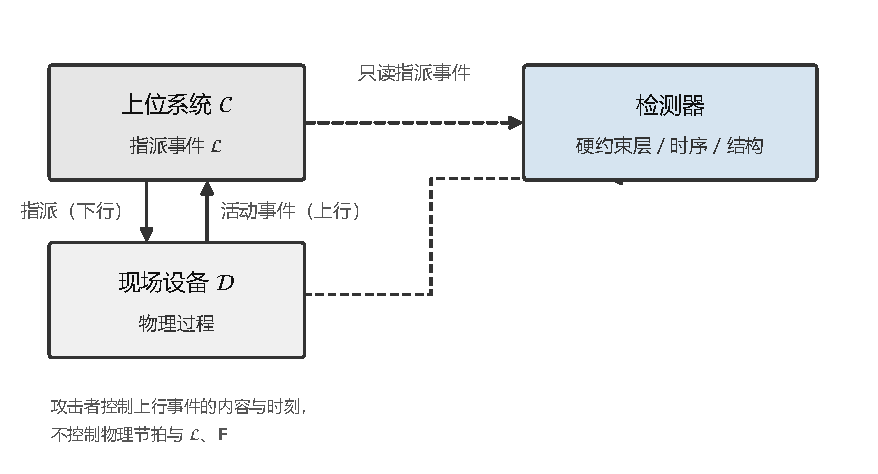
\includegraphics[width=0.92\linewidth]{figures/fig_system_CN.pdf}
\caption{指派/事件回环。检测器只读取同一日志中的指派事件与参考模型可行性掩码，对上行事件逐条作在线判决。}
\label{fig:system}
\Description{上位系统与现场设备构成指派下行、事件上行的回环，检测器只读指派事件并对上行事件作硬约束层、时序与结构三路判决。}
\end{figure}

\subsection{指派配对与可行性掩码}
\label{sec:ledger}

同一条事件日志也记录下行指派，其集合记为 $\mathcal{L}$。完成事件本应是某条指派的响应：若某条完成事件在对应的（设备，case）上不存在前置指派，则构成一步即可判定的因果缺失。智能工厂将流程管理与现场事件流双向集成后，该配对关系可直接从日志中读取~\cite{seiger2022factory}。指派--完成配对属于因果检查，而非时长检验：指派到开始之间的排队时延主要由设备竞争决定，不宜纳入时序通道。该检查作为硬约束层的实现细节保留，不单独评估（第~\ref{sec:hard}~节）。

可行性由随产线发布的参考过程模型（本文为 {BPMN}）导出，记为掩码 $\mathbf F$，包含两类硬约束。\emph{一元能力集}规定设备 $d$ 是否允许执行操作 $o$，不依赖前驱，因此覆盖全部消息。\emph{二元可达}规定在同一 case、同一设备上，能否从已确认的前驱操作 $o'$ 转移到 $o$。二者均无法从运行日志中学习得到：日志只记录历史上出现过的组合，无法区分``未曾观测''与``不允许''。同一份参考模型还可导出物料令牌守恒等跨设备约束（工件在工位间流转时，每次取用都应对应此前的一次放置），但在缺少工件级身份时，这类约束存在残余的良性违反，本文不将其纳入检测器（见第~\ref{sec:limitations}~节）。

\subsection{建模假设与威胁模型}
\label{sec:assumptions}

本文采用两项建模假设。第一，检测器只读取上行事件与同一日志中的指派，不评测上位系统据此如何派工。第二，参考模型与清洗后的正常日志一致，硬约束层在其上零违反；含错误执行的原始日志不满足该假设（表~\ref{tab:shift}）。

攻击者能力按 {Dolev--Yao} 模型~\cite{dolev1983yao}界定：攻击者作用于上行事件链路，可以窃听、重放、注入、丢弃或延迟消息，并可知道状态机结构乃至转移频率。攻击者可知检测器的结构与参数（含各分组的 $\sigma$），但不能观测检测器的在线状态（如 {CUSUM} 统计量与复位时刻）。攻击者不能攻破上位系统或设备固件，不能改变物理过程的推进速度，也不能改写日志中已写入的指派事件或参考模型。攻击目标是使事件记录与物理过程脱节。多设备协同伪造（需同时对齐多路事件与指派）不在本文范围之内。

\subsection{攻击类型}
\label{sec:coverage}

表~\ref{tab:inject}列出六类注入及其可复现规则。{A1} 朴素重放是重放攻击的基本对照。{A2} 物理不可行注入改写操作标签，使事件违反参考模型。{A3} 提前完成重放与 {A5} 渐变漂移不改动标签，只压缩停留时长：前者零散抽样，后者作用于一段连续活动。{A4} 状态模仿假设攻击者已知转移模型，插入最可能的下一步。{A6} 消息抑制删除整条尚未开始的活动。主要检测对象是 {A2} 与 {A3}/{A5}；{A1} 作为重放对照，{A4}/{A6} 用于界定检测能力的边界。

\begin{table}[!t]
\renewcommand{\arraystretch}{1.12}
\caption{六类注入的可复现规则。默认注入率 $20\%$，{A3}/{A5} 默认 $\rho=0.30$，三个注入种子；不改动 case。{A4} 须提供结构模型，否则将退化为重复当前操作，从而低估攻击者能力。评测默认不将同一实例的后续事件整体前移。}
\label{tab:inject}
\centering
\small
\begin{tabular}{llp{7.4cm}}
\toprule
编号 & 类型 & 规则 \\
\midrule
{A1} & 朴素重放 & 将该设备的一条历史活动在当前完成时刻之后重发；时长沿用历史值，标签形成重复。 \\
{A2} & 物理不可行注入 & 原地将操作名改写为该设备能力集之外（若无则改为其他操作）的标签；其后的良性事件会以伪造操作为前驱接受二元可达检查（下称级联比对）。 \\
{A3} & 提前完成重放 & 原地将完成时刻提前，使停留时长变为 $(1-\rho)\tau$；默认不平移同一实例的后续事件。 \\
{A4} & 状态模仿 & 已知模型：在当前完成之后插入转移概率最大的下一步，设备取日志中执行过该操作的设备，时长取该分组的中位数。 \\
{A5} & 渐变漂移 & 在时间序上取一段连续活动，对各条施加同一 $\rho$ 的停留压缩（区别于 {A3} 的零散抽样）。 \\
{A6} & 消息抑制 & 整条删除尚未开始的活动；标注于同一实例的后继事件上（可观测后果出现在下游）。 \\
\bottomrule
\end{tabular}
\end{table}

\subsection{检测问题}
\label{sec:detproblem}

\begin{problem}[离散事件注入检测]
\label{prob:detect}
给定仅含正常运行的历史日志、参考过程模型以及用户指定的误报预算 $\alpha$，对在线事件流逐条输出告警，以纯良性流上的逐消息告警率不超过 $\alpha$ 为目标；可交换时该目标由共形校准保证，时间序部署下的实测偏离见第~\ref{sec:boundary}~节。主要检测对象是 {A2} 与 {A3}/{A5}，{A1}/{A4}/{A6} 的结果一并报告。检测器不得使用攻击标签调整阈值。安全目标是\emph{可检出，或迫使伪造的相对提前量保持在较小范围}：单条伪造的相对提前量超过 $\rho^*(\alpha,\sigma)$ 后，被单消息检验检出的概率超过一半（第~\ref{sec:bound}~节）。
\end{problem}

评测指标有三项：同一 $\alpha$ 下延迟预算内的净检出率（检出率减去偶然告警基线，见第~\ref{sec:setup}~节）；以消息数计的检测延迟（箱线图，仅含预算内检出的注入）；纯良性流上的序贯误报率与告警间隔（告警次数过少时不据此估计 $\mathrm{ARL}_0$）。计算约束为每条消息 $O(1)$。

% ============================================================
%  第 4 章：方法
% ============================================================
\section{检测方法}
\label{sec:framework}

\subsection{总体架构}
\label{sec:arch}

生产配置由三路并行通道组成：硬约束层、结构通道与时序通道，任一通道触发即告警。离线阶段仅使用正常日志与参考模型：由 {BPMN} 导出 $\mathbf F$；按设备与操作估计转移概率与停留时长；在预留的校准折上以共形预测校准两路统计通道，并在良性流上为每路标定 {CUSUM} 门限 $h_i$，使该路平均误报间隔 $\mathrm{ARL}_{0,i}=1/\alpha_i$（$\alpha_i$ 为该路分得的预算，见下段）。在线阶段对每条消息执行常数次查表与对数运算，流程见图~\ref{fig:arch}与算法~\ref{alg:detect}。

误报预算在三路之间均分，每路 $\alpha_i=\alpha/3$：单消息门限取 $\alpha/3$，{CUSUM} 门限对应 $\mathrm{ARL}_{0,i}=3/\alpha$（$\alpha=0.01$ 时为 $300$）。三路以``或''合并后，整体单消息误报不超过 $\alpha$（{Bonferroni} 界），整体序贯告警率不超过各路之和，即整体 $\mathrm{ARL}_0$ 约不低于 $1/\alpha$。硬约束层在正常数据上的违反率为零，实际不消耗其份额，因此两个界均偏保守。并行判决的代价在于分摊：所有方法按子检测器数均分同一预算，仅标签消融只有一路、独享全部 $\alpha$，{BUTLA} 与 {HSMM} 各两路，{TABOR} 式三路；在仅有一路存在信号的攻击上，本文每路可用预算只有仅标签消融的三分之一。这一代价的实测影响见第~\ref{sec:e1}~节。

\begin{figure}[!t]
\centering
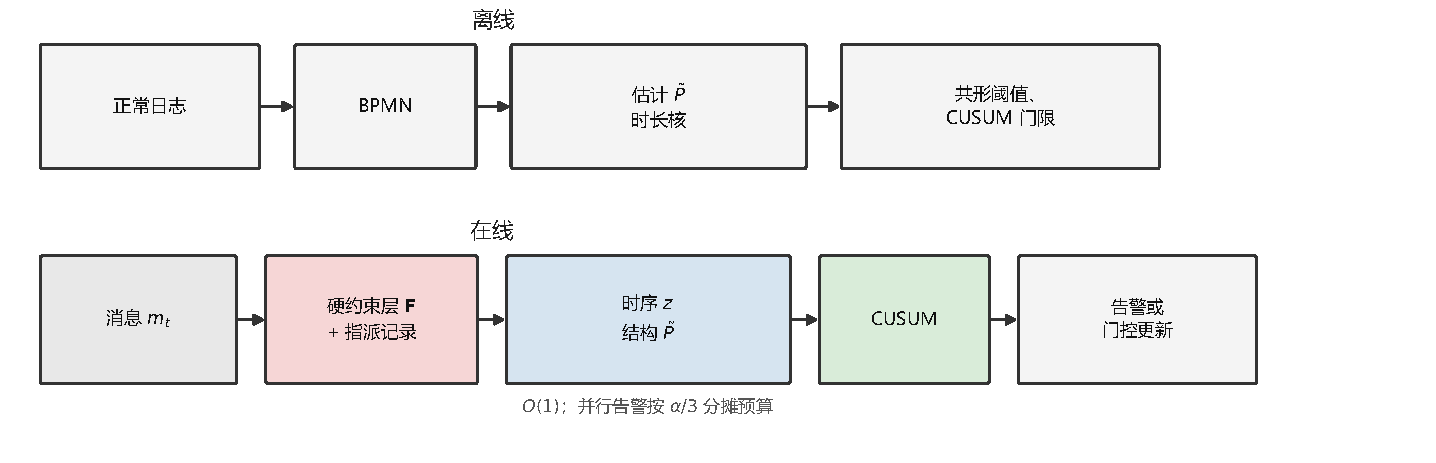
\includegraphics[width=0.98\linewidth]{figures/fig_arch_CN.pdf}
\caption{离线拟合与在线三路并行判决。硬约束层位于统计通道之前，以免不可行样本污染校准。}
\label{fig:arch}
\Description{离线阶段由日志与BPMN估计转移、时长核并校准阈值；在线阶段对每条消息依次做硬约束层否决、时序与结构打分及CUSUM累积。}
\end{figure}

硬约束层须置于最前：其判决不产生误报、结果可解释，并可避免不可行样本进入后续校准。结构通道与时序通道并列而非串联，以同时覆盖``标签错误''与``标签正确但时间错位''两类情形。序贯检验置于最后，因此两路统计通道必须输出连续分数，而不是布尔判决。

\begin{algorithm}[!t]
\caption{离散事件注入的在线检测}
\label{alg:detect}
\begin{algorithmic}[1]
\Require 事件 $m=(d,o,t)$；指派 $\mathcal{L}$；掩码 $\mathbf{F}$；核 $(\tilde P,\mu,\sigma)$；共形校准器；门限 $h$
\Ensure 告警或接受
\If{一元能力、二元可达或指派--完成任一违反}
    \State \textbf{return} 告警（硬约束层原因）
\EndIf
\State 计算时序残差 $z$ 与结构分数 $\tilde P_{o'\to o}$
\State 用冻结的共形校准器把两路分数分别转换为共形 $p$ 值 $p$
\State 对两路分别更新 $S\leftarrow\max(0,\,S-\log p-c)$
\If{任一路 $S\ge h$}
    \State 复位该路；\textbf{return} 告警
\EndIf
\If{隔离窗口内无告警}
    \State 门控更新 $(\mu,\sigma)$ 并锚定状态
\EndIf
\State \textbf{return} 接受
\end{algorithmic}
\end{algorithm}

图~\ref{fig:alarm}逐条解析两个真实案例。{A2} 由一元能力集立即否决，并给出可读的告警原因；{A3} 的标签完全合法，其落在区间守卫内侧的负残差经 {CUSUM} 累积后越过门限。

\begin{figure}[!t]
\centering
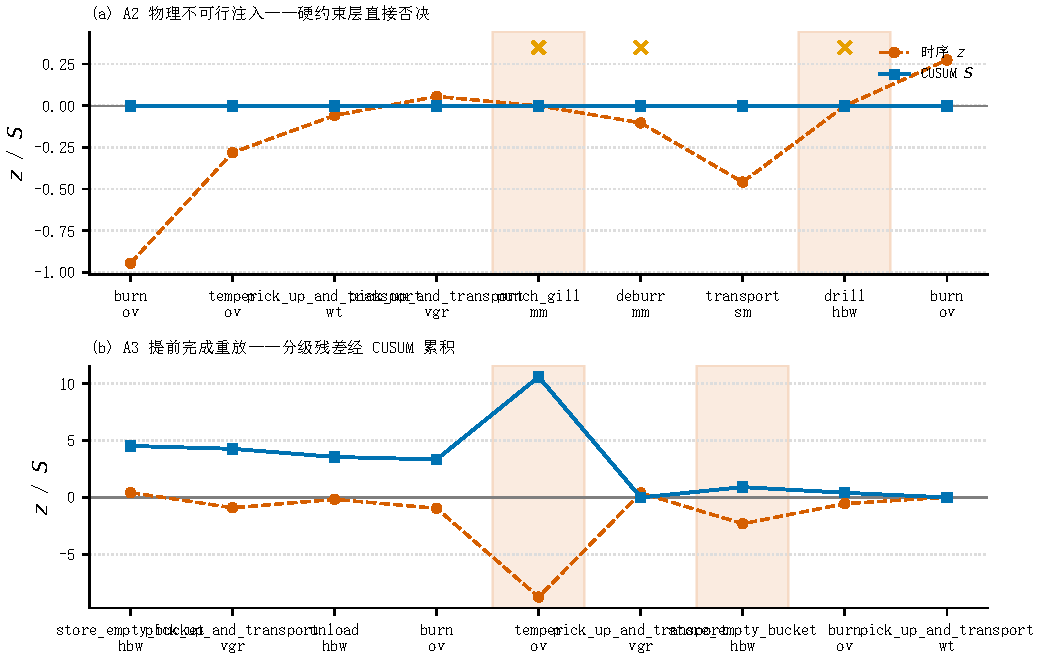
\includegraphics[width=0.98\linewidth]{figures/fig_alarm_CN.pdf}
\caption{{A2} 硬约束层否决与 {A3} 时序证据累积的逐条解析。阴影列为注入消息；叉号表示硬约束层触发。}
\label{fig:alarm}
\Description{上下两行为逐条解析：上行 A2 在注入处被硬约束层否决；下行 A3 的时序残差为负，CUSUM 随后越过门限。}
\end{figure}

\subsection{硬约束层}
\label{sec:hard}

对消息 $(d,o,t)$，硬约束层依次检查三项，任一失败立即告警并给出原因。
\begin{enumerate}[leftmargin=1.4em,itemsep=2pt]
\item 一元：$(d,o)$ 是否属于参考模型的能力集。
\item 二元：若同一 $(d,\mathrm{case})$ 存在已确认前驱 $o'$，则 $(o'\to o)$ 是否被 $\mathbf F$ 允许。
\item 因果：该完成事件是否存在前置指派事件。
\end{enumerate}
掩码由随数据集发布的 {BPMN} 自动导出：一元能力集取自节点上绑定的设备类型（或资源角色），二元可达关系由同一工作流内的顺序结构与网关展开得到，无需手工编写转移表。一元检查覆盖全部消息，在正常数据上的违反率为零。参考模型的价值在时间序划分下尤为明显：测试折中有 $20/508$（$3.9\%$）的良性活动属于训练折中未出现的（设备，操作）组合，比例远高于 $\alpha=0.01$，若按``训练数据中未出现即异常''判决将产生大量误报，而参考模型对其中 $0$ 条作出拒绝。第三项因果检查属实现细节：六类注入均不破坏指派--完成配对，本文不单独评估该项，也不将其计入贡献。

\subsection{结构通道}
\label{sec:struct}

结构通道判定当前活动在 case 级工作流序列上是否常见。链的粒度取 case，而非（设备，case）：本日志中的设备均为被调用的服务端点，按设备切分的事件链大多长度为~$1$，转移概率缺乏区分度。通道状态取操作名，而非（设备，操作）：``错误的设备执行了正确的操作''已由一元能力集覆盖，不应再由统计通道对未出现的组合赋予过小的概率，因为在时间序划分下，良性数据本身就会产生新组合（改取（设备，操作）的实测代价见第~\ref{sec:e2}~节）。转移概率采用浓度参数为 $0.5$（{Jeffreys} 型）的对称 {Dirichlet} 后验预测 $\tilde P$，以避免小样本导致的伪零，同时保留由 $\mathbf F$ 强制的真零。

输入共形校准器的分数是预测概率 $\tilde P_{o'\to o}$ 本身，理由见第~\ref{sec:conformal}~节。case 的首条活动没有前驱，结构通道对其弃权，分数按最不异常计。该通道对 {A4}/{A6} 这类改变事件数目的攻击较为敏感。

\subsection{半马尔可夫时序通道}
\label{sec:timing}

半马尔可夫核写作 $Q_{o'o}(\tau)=P_{o'o}F_{o'o}(\tau)$。停留时长按（设备，操作）分组，取 $\log\tau\sim\mathcal{N}(\mu,\sigma^2)$。与计时自动机的差别在于 $F_{o'o}$ 是概率分布而非区间守卫，见第~\ref{sec:md}~节。位置参数 $\mu$ 按行驶路线（起止库位）作加性分解：同一分组内观测不少于 $8$ 条的路线取自己的效应，其余并入分组的共同截距；未见路线回落为计划时长加该分组的系统偏差。训练折中未出现或观测少于 $2$ 条的分组，以及下文所述的弃权分组，时序通道不给出证据，分数按最不异常计；测试折 $508$ 条活动中共 $56$ 条（$11.0\%$）属于此类。

四种观测对应四个分支。
\begin{itemize}[leftmargin=1.4em,itemsep=2pt]
\item \textbf{状态跳变。} 标准化残差 $z=(\log\tau-\mu)/\sigma$，仅作左侧检验（停留时长过短即为提前上报）。提前上报对应有方向的备择假设；采用单侧检验的价值主要在于阈值稳定，而非功效成倍提升。
\item \textbf{同状态心跳。} 右删失生存函数 $-\log\bigl(1-F(\tau)\bigr)$，仅在停留时长过长时告警。
\item \textbf{超时无消息。} 采用同一生存函数，由超时看门狗在停留时长超过该分组对数正态模型的 $99.9\%$ 分位时触发。该分支可覆盖``活动已开始但完成事件被抑制''的情形，而无法覆盖``活动整条从未开始''的情形，后者需要活动间隔模型，本文不提供。
\item \textbf{周期轮询。} 区间删失 $\log\bigl[F(\tau+\Delta)-F(\tau)\bigr]$，以免量化误差污染似然。主实验为事件驱动日志，该分支不参与评测。
\end{itemize}
时序通道的不符合度分数取 $-z$（取值越大越异常），而不取参数化 $p$ 值，理由见第~\ref{sec:conformal}~节。人工工位的 $\sigma$ 可接近~$2$；对人工工位及 $\sigma\ge1$ 的分组（此时 $\alpha=0.01$ 下 $\rho^*>90\%$），时序通道直接弃权。整体检测能力由变异最大的工序决定。

\subsection{共形校准与序贯累积}
\label{sec:conformal}

两路统计通道在留出的正常样本上做分割共形预测~\cite{shafer2008conformal,angelopoulos2023conformal}：对每条新消息，以其不符合度分数在校准分数中的排名给出共形 $p$ 值 $p_t$。校准数据与部署数据可交换时，$p_t$ 在良性流上服从均匀分布，按 $p_t\le\alpha/3$ 判决即可保证单通道误报不超过 $\alpha/3$。该保证不依赖高斯或马尔可夫假设，但依赖可交换性~\cite{barber2023exchangeability}。部署阶段只能按时间先后划分数据，可交换性并不自动成立，本文因此另行报告时间序划分下的经验误报率（第~\ref{sec:boundary}~节）。有限校准集可达的最低单消息误报水平约为 $1/(n+1)$，$n$ 为校准样本数；本文不把单消息 $\alpha$ 设得低于 $10^{-2}$，更低的误报预算由 {CUSUM} 的 $\mathrm{ARL}_0$ 承担。

不符合度分数必须在尾部保持单调次序，因此两路通道都直接输入原始分数，而不输入参数化或随机化的 $p$ 值。时序通道输入 $-z$：参数化 $p$ 值在 $10^{-12}$ 处截断后，良性失配与明显的提前上报会被压缩为同一取值，尾部次序随之丢失。结构通道输入 $\tilde P$：随机化概率积分变换会把 {Dirichlet} 平滑产生的大量并列取值摊成一个均匀区间，使从未出现过的转移约有一半机会得到高于 $\alpha$ 的 $p$ 值。共形 $p$ 值自身带有随机化项，并列情形只在这一步打破一次。两项选择的实测影响见第~\ref{sec:e2}~节。

对每路通道的共形 $p$ 值做单侧 {CUSUM}~\cite{li2015quickest}：
\begin{equation}
  S_t=\max\bigl(0,\,S_{t-1}-\log p_t-c\bigr),
  \label{eq:cusum}
\end{equation}
其中 $-\log p_t$ 是第 $t$ 条消息提供的证据量，提前上报等异常使 $p_t$ 偏小、证据量增大。良性流上 $p_t$ 服从均匀分布，$-\log p_t$ 服从均值为~$1$ 的指数分布，因此参考值 $c$ 必须大于~$1$，统计量才不会在良性流上无界增长；本文取 $c=1.5$。$S_t$ 越过门限 $h$ 即告警，$h$ 在良性流上逐路标定，使该路 $\mathrm{ARL}_{0,i}=1/\alpha_i$（三路时为 $3/\alpha$）。告警后必须复位，否则统计量将持续停留在门限之上，导致后续每条消息均触发告警。所有输出连续分数的基线均采用同一累积规则，以免将增益误归因于 {CUSUM} 本身。

\subsection{门控更新与复杂度}
\label{sec:online}

各链的前驱状态逐条推进。时长模型以遗忘因子 $0.95$ 的指数滑动平均缓慢更新所在分组的 $(\mu,\sigma)$；结构通道的 $\tilde P$ 不在线更新。更新必须门控：只有当该消息通过全部通道、且不处于隔离窗口（最近一次告警之后的 $20$ 条消息）之内时，才允许进入基线；否则攻击者可以通过持续的小幅提前上报，逐步把时长基线拉向伪造值。门控的实测效果见第~\ref{sec:gate}~节。主表与消融实验均关闭在线更新，使用冻结的模型；门控与时延实验沿用同一判决协议（三路、每路 $\alpha/3$、逐路 {CUSUM}），仅开启门控更新。

单条消息的计算复杂度为 $O(1)$：常数次查表、对数运算与硬约束层判断，在热路径上与状态数、设备数无关。多设备可按链并行处理。第~\ref{sec:e8}~节给出常数因子。

% ============================================================
%  第 5 章：理论分析
% ============================================================
\section{理论分析}
\label{sec:theory}

\subsection{仅标签检测族对标签自洽注入的不可能性}
\label{sec:ta}

考虑一类仅使用标签的检测器，下称仅标签检测族：由前驱 $i$ 得到预测分布 $\hat{\mathbf p}$，将观测记为独热向量 $\mathbf e_j$，以 $\delta(i,j)=\|\mathbf e_j-\hat{\mathbf p}\|_2$ 或任一随 $p_j$ 严格单调递减的量与自适应阈值比较。设预测分布满足：$p_j=0$ 当且仅当转移 $i\to j$ 被可行性掩码 $\mathbf F$ 禁止，即预测器采用平滑估计，不因样本不足产生伪零（第~\ref{sec:struct}~节的 {Dirichlet} 后验预测满足该条件）。展开
\begin{equation}
  \delta(i,j)^2=1-2p_j+\|\hat{\mathbf p}\|^2
\end{equation}
可见 $\|\hat{\mathbf p}\|^2$ 对同一前驱 $i$ 下的所有 $j$ 均为常数，$\delta$ 只是 $p_j$ 的单调变换，几何形式不提供额外信息。

因此 $\delta$ 是 $(i,j)$ 的确定性函数，与该消息是良性还是注入无关。记 $q_{ij}$ 为良性流中前驱 $i$ 之后出现 $j$ 的真实频率，$\mathrm{FPR}_i$ 为前驱 $i$ 之后良性消息上的误报率。

\begin{proposition}[仅标签检测族的不可能性]
\label{prop:ta}
设检测器对前驱 $i$ 之后的观测 $j$ 只依据 $(i,j)$ 判决，且判决为 $p_j$ 的单调函数；并设 $q_{ij}=0$ 当且仅当 $i\to j$ 被 $\mathbf F$ 禁止。则：
(i) 在零误报约束下，可标记的转移恰为被 $\mathbf F$ 禁止的转移，对标签自洽的注入，该检测族相对掩码的增量为零；
(ii) 对不改动标签的注入，每条消息的单消息判决与其良性版本相同；若注入也不改变消息次序，序贯判决同样相同，净检出为零，与 $\alpha$ 无关。
\end{proposition}

\begin{proof}
(i) 若某个 $q_{ij}>0$ 的 $j$ 被标记，则每一次良性出现的 $j$ 都触发告警，$\mathrm{FPR}_i\ge q_{ij}>0$，与零误报矛盾；故只有 $q_{ij}=0$、即被 $\mathbf F$ 禁止的转移可被标记。(ii) 标签不变时每条消息的 $(i,j)$ 不变，判决随之不变；次序也不变时分数序列与良性版本逐条相同，告警位置相同，检出只来自偶然告警。
\end{proof}

攻击者的最优规避选择为 $\arg\min_j\delta_j=\arg\max_j p_j$，即日志中最常见、伪造后最接近正常行为的下一步。

该结论不依赖具体的阈值系数：凡判决仅为预测概率的一元函数的检测器，均属于该族。命题~\ref{prop:ta}(ii) 预测一阶马尔可夫消融在纯时序攻击 {A3}/{A5} 上的净检出为零；第~\ref{sec:e1}~节实测扣除偶然告警基线后为 $-0.01$ 与 $0.00$，与预测一致。

\subsection{分布型时长与时钟守卫}
\label{sec:md}

计时自动机对转移 $(o',o)$ 给出时钟守卫 $[\ell,u]$：停留时长 $\tau\in[\ell,u]$ 则接受，否则拒绝~\cite{maier2011timed,lin2018tabor}。若攻击者把一次正常停留 $\tau$ 缩短为 $(1-\rho)\tau$，而 $(1-\rho)\tau$ 仍落在 $[\ell,u]$ 之内，则单步判决为正常。由于守卫是二值判断，同一方向上多次略偏快的停留不会被累积。

半马尔可夫通道输出的是连续残差 $z=(\log\tau-\mu)/\sigma$。提前上报使 $\mathbb{E}[z]=\log(1-\rho)/\sigma<0$，对应的共形 $p$ 值系统性偏小，证据量 $-\log p_t$ 的均值随之增大。良性流上 $\mathbb{E}[-\log p_t]=1<c$；只有当位移足够大、使 $\mathbb{E}[-\log p_t]>c$ 时，{CUSUM} 统计量才以正漂移越过 $h$，即使每条观测单独都未越过单消息阈值。位移较小时统计量没有正漂移，只能靠波动偶然越过门限，这与表~\ref{tab:e4}中小 $\rho$ 下的低检出相对应。这一差别不在于是否对停留时长建模，而在于\emph{证据形态}：区间守卫将落在区间之内的提前上报映射为零，分布型残差则将其映射为可加的增量。图~\ref{fig:guard}给出示意：全部观测落在守卫之内，二值通道不告警，{CUSUM} 仍越过门限。{A3} 正是这一差别的典型情形：其标签完全合法，计时自动机予以接受，而序贯半马尔可夫检验仍可能检出。

\begin{figure}[!t]
\centering
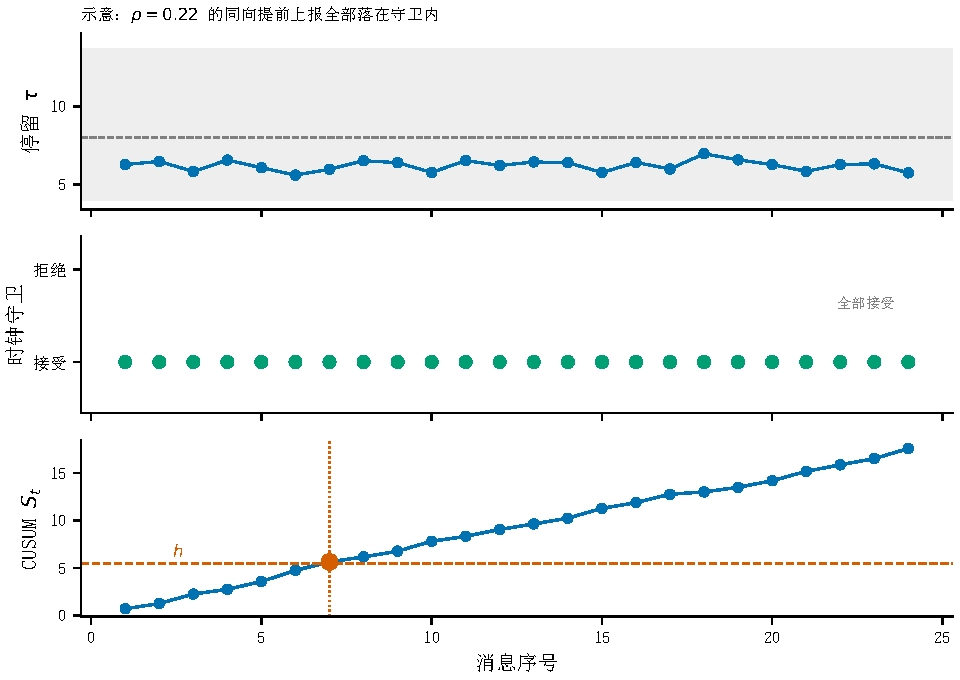
\includegraphics[width=0.95\linewidth]{figures/fig_guard_cusum_CN.pdf}
\caption{时钟守卫与分布型残差的差别（示意，非评测轨迹）。灰色带为区间守卫；同向提前上报全部被接受，{CUSUM} 仍累积越过 $h$。}
\label{fig:guard}
\Description{三行示意：停留时长均落在灰色守卫带内，时钟守卫全部接受，CUSUM 统计量随后越过门限。}
\end{figure}

\subsection{临界相对提前量}
\label{sec:bound}

本节给出单消息检验下伪造停留时长的临界缩短比例。考虑单消息左侧检验：残差低于阈值 $-z_{1-\alpha}$ 即告警。攻击者把停留时长缩为 $(1-\rho)\tau$ 后，残差分布整体左移；当左移量使残差均值恰好落在阈值上时，单条伪造消息被检出的概率为 $1/2$。攻击者若希望每条伪造以过半概率逃过检验，相对提前量就不能超过这一临界值，本文称之为临界相对提前量 $\rho^*$。它不是规避量的严格上界：$\rho<\rho^*$ 的伪造仍以低于一半的概率被检出，序贯累积还会进一步提高检出。

\begin{proposition}[临界相对提前量]
\label{prop:rho}
设正常停留满足 $\log\tau\sim\mathcal{N}(\mu,\sigma^2)$，左侧水平为 $\alpha$，阈值为 $-z_{1-\alpha}$。攻击将观测时长缩为 $(1-\rho)\tau$。使攻击后残差均值恰好落在阈值上的相对提前量为
\begin{equation}
  \rho^*(\alpha,\sigma)=1-e^{-\sigma z_{1-\alpha}}.
  \label{eq:rho}
\end{equation}
若检验作用于 $k$ 条独立伪造残差的均值，其标准差按 $1/\sqrt{k}$ 收缩，
\begin{equation}
  \rho^*_k(\alpha,\sigma)\approx 1-e^{-\sigma z_{1-\alpha}/\sqrt{k}}.
  \label{eq:rhok}
\end{equation}
\end{proposition}

\begin{proof}
对数域位移 $\Delta=\log(1-\rho)$，标准化后均值移动 $\Delta/\sigma$。令 $\Delta/\sigma=-z_{1-\alpha}$，解出 $\rho=1-e^{-\sigma z_{1-\alpha}}$。对 $k$ 条独立残差取均值把 $\sigma$ 换成 $\sigma/\sqrt{k}$，即得式~\eqref{eq:rhok}。
\end{proof}

式~\eqref{eq:rho}只包含时序变异与误报预算，不含系统矩阵。它是隐蔽攻击基本极限~\cite{liu2022limits}在离散事件场景下的实例：结论形式并不新颖，新的是实例化对象为相对提前量，而不是连续状态偏差的能量。式~\eqref{eq:rhok}给出重复注入下的收紧结果；本文实验只验证单次注入，不把 $\sqrt{k}$ 收缩作为已验证的结论。

上述 $1/2$ 点对应\emph{单一}高斯分布。产线各工序的 $\sigma$ 高度异质，低变异分组在远小于全局 $\rho^*$ 的相对提前量下即可被检出，因此按工序混合后的整体检出率曲线（下称混合功效曲线）在 $\rho<\rho^*$ 时就可以明显高于 $1/2$。第~\ref{sec:e4}~节验证的是这条混合曲线与实测结果的吻合程度。图~\ref{fig:sigma}给出 $\rho^*$ 随 $\sigma$ 的变化：全局 $\sigma=0.236$ 对应 $42.2\%$；人工工位的 $\sigma$ 接近~$2$ 时 $\rho^*$ 趋近于~$1$，检验失去区分力，产线整体的可检测性由变异最大的工序决定。第~\ref{sec:e4}~节按 $\alpha=0.01$ 的单通道检验验证；三路配置中时序通道分得 $\alpha/3$，$\sigma=0.236$ 时对应 $\rho^*=47.3\%$。

\begin{figure}[!t]
\centering
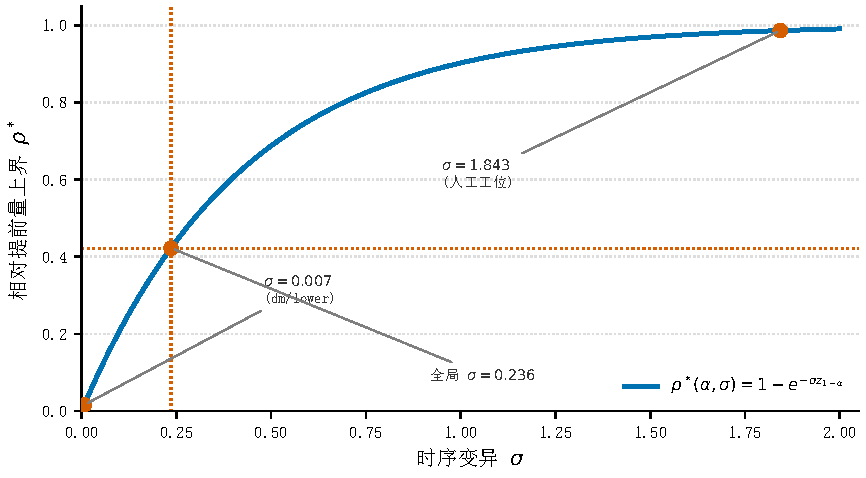
\includegraphics[width=0.82\linewidth]{figures/fig_sigma_CN.pdf}
\caption{$\alpha=0.01$ 单侧下 $\rho^*$ 随 $\sigma$ 的变化。标注点为低变异工序、全局加权 $\sigma$ 与人工工位。}
\label{fig:sigma}
\Description{临界相对提前量随时序变异增大并趋近于一，全局 sigma 为 0.236 时 rho 星约百分之四十二。}
\end{figure}

% ============================================================
%  第 6 章：实验
% ============================================================
\section{实验与结果分析}
\label{sec:experiments}

\subsection{实验设置}
\label{sec:setup}

主数据采用 {University of Trier} 教学工厂发布的 {Fischertechnik} 智能工厂 {IoT} 事件日志~\cite{malburg2022trier}。选用该日志，是因为它是目前少有的同时提供 {BPMN} 参考模型与指派--执行--完成生命周期的公开活动日志，而非因其规模具有代表性。{HAI} 等 1~Hz 过程量数据集无法实例化指派与工序活动~\cite{shin2020hai}，工业控制系统测试床与公开数据集的综述也以过程量与网络流量为主~\cite{conti2021testbeds,dobler2025datasets}，因此本文不报告跨数据集结果。清洗后全日志共 $3{,}062$ 条活动，产线上十余台设备均为被调用的服务端点。

日志内部的多样性用于压力测试，不替代第二份外部数据：随数据发布的 {BPMN} 共 $16$ 个；官方含错版本（含 NTP 时钟漂移、重复与缺失记录）用于误报压力测试；时间序测试折包含训练折中未出现的五个工作流。可行性掩码 $\mathbf F$ 按第~\ref{sec:hard}~节的规则由 {BPMN} 自动导出。

公开活动日志不含注入标注~\cite{conti2021testbeds,dobler2025datasets}。本文将 {Dolev--Yao} 模型中的重放、注入与丢弃映射到本日志的字段上，规则见表~\ref{tab:inject}，注入器随代码发布。数据按时间先后划分为互不重叠的拟合折（$1{,}951$ 条）、校准折（$603$ 条）与测试折（$508$ 条良性事件），注入只在测试折上实施。主表注入率为 $20\%$，并扫描 $5\%/10\%/20\%/40\%$；相对提前量默认 $\rho=0.30$。样本结构为 $1$ 份日志 $\times$ $1$ 次时间序划分 $\times$ $6$ 类攻击 $\times$ $3$ 个注入种子；注入种子（$0,1,2$）只决定注入位置，不重新划分数据，检测器的拟合种子固定为 $0$。三个种子合计，每类攻击注入 $297$ 条（{A1} 为 $290$ 条，{A2} 为 $303$ 条，{A6} 为 $201$ 条），同一种子下各方法面对同一条受攻击流。第~\ref{sec:e4}~节的相对提前量扫描另采用按分组分层抽取的校准集（$n_{\mathrm{cal}}=701$），以保证每个（设备，操作）分组都有足够的校准样本。检测延迟按注入实例存档，箱线图仅含预算内检出的实例。全部实验在单机（{Intel Xeon W-1270}，$64$~GB 内存）上以 {Python}~3.7.6、{NumPy}~1.18.1、{SciPy}~1.4.1 运行。

三条主基线均按原文的结构约束复现，而不是使用官方代码：{BUTLA} 与 {TABOR} 未随文发布可对接本日志格式的实现，隐半马尔可夫模型（{HSMM}）属于模型类而非工业检测器。表~\ref{tab:repro}列出复现中保留的结构与所作近似。所有输出连续分数的方法都套用同一 {CUSUM}（参考值 $c=1.5$，延迟预算 $10$ 条消息，告警后复位）。每个方法的误报预算在其子检测器之间均分，分得 $\alpha_i$ 的子检测器按 $\mathrm{ARL}_0=1/\alpha_i$ 标定门限 $h$：仅标签消融 $1$ 路，{B1}/{B3} 各 $2$ 路，{B2} 与本文各 $3$ 路。为使各方法在相同误报水平下比较，主表中的阈值与 {CUSUM} 门限均在测试折的未注入版本上标定，使经验误报对齐到 $\alpha$。该设置不使用攻击标签，也不使用受攻击流内部的良性事件，但借用了测试折的良性分布，属于理想化标定。部署时门限只能取自校准折，为此另以校准折为参照流重跑全部方法；此时各方法的误报不再对齐，其检出与测试折误报一并在第~\ref{sec:e1}~节报告。本文方法与各基线同样只用拟合折拟合。主表中本文三路通道的原始分数与基线分数经同一判决流程（参照流上的经验 $p$ 值与上述 {CUSUM}）处理，不经过冻结的共形校准器，以免比较中混入两套阈值机制；含共形校准器的逐通道经验误报见第~\ref{sec:boundary}~节。仅标签的一阶马尔可夫似然是去掉时间维度的消融配置，而不是独立的先行方法。参考模型符合度代理（违反 $\mathbf F$ 即告警）与硬约束层判决相同，不在主表中单列，其单消息结果即表~\ref{tab:coverage}的硬约束层列。

\begin{table}[!t]
\renewcommand{\arraystretch}{1.12}
\caption{主基线的复现协议。对照的是原文结构约束，不是官方二进制。}
\label{tab:repro}
\centering
\small
\begin{tabular}{lp{3.4cm}p{4.4cm}}
\toprule
方法 & 保留 & 本日志上的近似 \\
\midrule
{B1} {BUTLA} 式~\cite{maier2011timed}
  & 按组件各学一台自动机；无跨组件检查；时长为偏离容差
  & 组件取为设备；容差改为同 $\alpha$ 下的经验分位，以免将误报差异误计为方法差异 \\
{B2} {TABOR} 式~\cite{lin2018tabor}
  & 工段内依赖；不使用指派（命令）数据
  & 工段取为设备；工段内采用 $P(o)\prod P(v\mid o)$（与饱和联合分布的对照见表后） \\
{B3} {HSMM}~\cite{tan2008hsmm}
  & 显式时长的半马尔可夫模型
  & 观测为操作与 $\log\tau$；$K\in\{2,3,4,6\}$ 由留出似然选定为 $6$ \\
\bottomrule
\end{tabular}
\end{table}

原文学到的工段内结构介于朴素分解与饱和联合分布 $P(o,v_1,\dots,v_m)$ 之间。在主表协议下将 {B2} 的工段内分布换为饱和联合分布后，六类均值由 $0.21$ 变为 $0.22$，{A3} 上由 $0.10$ 变为 $0.08$，本文在六类攻击上仍均高于该变体。

在延迟预算内采用``窗口中出现任一告警即判为检出''的判定规则时，即使检测器不具备任何真实检测能力，窗口内的随机误报也会带来一定的检出率。该偶然告警基线为 $1-(1-\mathrm{FPR})^{B+1}$，其中 $B=10$ 为延迟预算。表中主结果均已扣除该基线，未扣除的数值不单独引用。逐消息检出率受参照流长度限制，在本规模下不作为主结果。

方法间比较以注入实例为配对单位：同一种子下各方法面对同一条受攻击流，逐条注入记录其是否在延迟预算内被检出，对每类攻击上本文与每个对照方法的差异做双侧精确 {McNemar} 检验，并按注入实例做 $2{,}000$ 次自助重抽样，给出检出率差的 $95\%$ 置信区间。$6$ 类攻击与 $4$ 个对照共 $24$ 个比较，按 {Holm} 法校正。该检验针对未扣除偶然告警基线的原始检出；同一受攻击流内的注入按相互独立处理，这是一项近似。

\subsection{单通道覆盖诊断}
\label{sec:diag}

在端到端对照之前，表~\ref{tab:coverage}先给出三路通道各自的单消息检出率，以说明各类攻击由哪一路负责。{A2} 由一元能力集拒绝，时序通道对其不敏感。{A3}/{A5} 不改动标签，仅压缩停留时长，硬约束层与结构通道的检出接近于零，时序通道是唯一有实质检出的通道。{A1} 沿用历史时长，时序通道无增益，检出由硬约束层与结构通道承担。{A4} 按转移模型插入概率最大的下一步，三路通道的单消息检出均接近误报水平。{A6} 删除整条尚未开始的活动，超时看门狗不会被触发，结构通道只在下游有微弱信号。图~\ref{fig:coverage}将同一张表绘制为相对误报的净提升热图。

表~\ref{tab:coverage}的数字不能与后文表~\ref{tab:e1}直接比较：前者是单通道、单消息、未分摊误报预算且未扣除偶然告警基线的诊断；后者是三路并行、每路预算 $\alpha/3$、延迟预算 $10$ 条消息且扣除偶然告警基线后的端到端净检出。例如 {A3} 的时序单消息检出为 $0.43$，而表~\ref{tab:e1}中为 $0.18$，二者并不矛盾。

\begin{table}[!t]
\renewcommand{\arraystretch}{1.15}
\caption{三路生产通道对六类注入的单消息检出率，括号内为同一批良性事件上的误报。各通道单独以 $\alpha=0.01$ 判决，冻结模型，测试折 $508$ 条，注入率 $20\%$，三个注入种子均值。{A2} 硬约束层的 $0.06$ 并非纯良性误报，而是级联比对所致：注入后的下一条良性事件以伪造操作为前驱，因而被二元可达检查拒绝。其部署语义为``已检出攻击，但归因于后一条事件''，故与第~\ref{sec:e1}~节的纯良性流误报分开报告。}
\label{tab:coverage}
\centering
\small
\begin{tabular}{llccc}
\toprule
编号 & 类型 & 硬约束层 $\mathbf F$ & 结构 & 时序 \\
\midrule
{A1} & 朴素重放 & $0.22\,(0.00)$ & $0.21\,(0.02)$ & $0.03\,(0.02)$ \\
{A2} & 物理不可行注入 & $0.98\,(0.06)$ & $0.29\,(0.02)$ & $0.00\,(0.02)$ \\
{A3} & 提前完成重放 & $0.00\,(0.00)$ & $0.02\,(0.01)$ & $0.43\,(0.02)$ \\
{A4} & 状态模仿（已知模型） & $0.03\,(0.00)$ & $0.01\,(0.01)$ & $0.00\,(0.02)$ \\
{A5} & 渐变漂移 & $0.00\,(0.00)$ & $0.01\,(0.01)$ & $0.48\,(0.03)$ \\
{A6} & 消息抑制 & $0.00\,(0.00)$ & $0.16\,(0.01)$ & $0.04\,(0.02)$ \\
\bottomrule
\end{tabular}
\end{table}

\begin{figure}[!t]
\centering
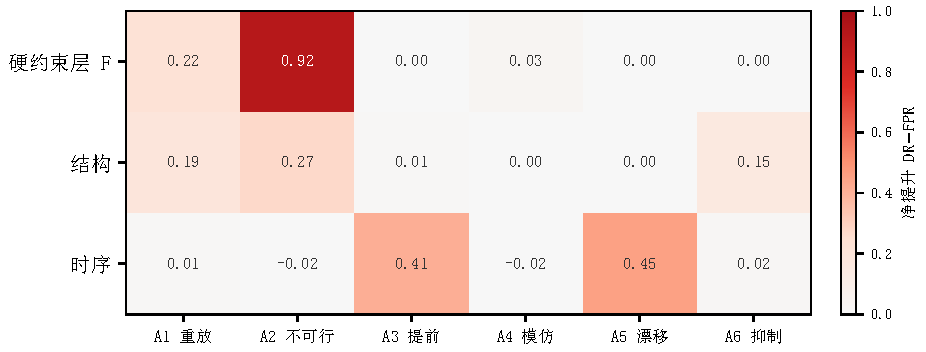
\includegraphics[width=0.98\linewidth]{figures/fig_coverage_CN.pdf}
\caption{三路生产通道相对良性误报的净提升（{DR}$-${FPR}）。{A2} 由硬约束层覆盖，{A3}/{A5} 仅时序通道有实质提升，{A4} 不存在专属通道。}
\label{fig:coverage}
\Description{三行六列热图：硬约束层、结构、时序对 A1 至 A6 的净检出提升，A2 硬约束层与 A3、A5 时序为深色高值，A4 接近零。}
\end{figure}

\subsection{与计时自动机及半马尔可夫模型的对照}
\label{sec:e1}

表~\ref{tab:e1}给出 $\alpha=0.01$ 下的净检出率。本文方法在六类攻击上的均值为 $0.48$，{B1}/{B2}/{B3} 分别为 $0.17/0.21/0.11$。下面分三类攻击说明。

第一，纯时序攻击。{A3}/{A5} 不改动标签，仅标签消融扣除偶然告警基线后为 $-0.01$ 与 $0.00$，即其分数流与良性流逐条相同，与命题~\ref{prop:ta}(ii) 一致。{A5} 上本文为 $0.87$，是差距最明显的一项；计时自动机类基线同样能捕捉累积式漂移（$0.59/0.48$），但仍低于按（设备，操作）作左尾检验的分布型通道。{A3} 上本文为 $0.18{\pm}0.01$，{B1}/{B2} 为 $0.10{\pm}0.03$ 与 $0.10{\pm}0.04$。逐注入配对检验下，本文对 {B1} 的检出率差为 $0.067$（$95\%$ 区间 $[0.020,0.114]$，Holm 校正 $p=0.031$），对 {B2} 为 $0.064$（$[0.010,0.118]$，校正后 $p=0.096$，不显著）；增益幅度有限，其来源是零散的提前上报在分布型残差下仍可累积。{B3} 在 {A3} 上仅为 $0.06$，说明增益并非单纯来自``半马尔可夫模型对区间守卫''的模型类差异：{HSMM} 的时长核绑定在隐状态上，标签未改的提前上报被吸收为一次略短的停留。

第二，重放与不可行注入。{A1}/{A2} 上本文为 $0.55/0.95$，高于三条主基线（配对检验经 Holm 校正，$p$ 均小于 $10^{-20}$）。{A2} 由一元能力集覆盖，{B2} 的工段内依赖无法替代参考模型。{B2} 与 {B1} 在多数攻击族上表现接近：工段内依赖在本日志上信息量较低，而且 {B2} 对``该设备从未执行过此操作''赋予的极端分数，在良性测试折中就已出现（即第~\ref{sec:hard}~节所述的未出现组合），参考模型则不会拒绝这些组合。

第三，改变事件数目的攻击。{A4}/{A6} 上本文为 $0.17/0.14$，低于仅标签消融的 $0.23/0.28$（Holm 校正 $p=0.001$ 与 $p<10^{-6}$）。这两类攻击主要由结构通道负责；三路均分后结构通道只获得 $\alpha/3$，而仅标签消融以单路独享 $\alpha$，预算分摊是与之相符的解释。本文将这一差距作为多通道设计的代价报告，不作为主结论。在 $\alpha=0.05$ 下，{A4}/{A6} 上本文（$0.18/0.19$）仍低于仅标签消融（$0.41/0.45$），说明该劣势并非由 $\alpha=0.01$ 时的校准分辨率不足所致；但排序并非全部不变，{A1} 上本文此时也低于仅标签消融（$0.47$ 对 $0.61$）。

{B3} 的 {EM} 似然单调收敛，时长核非退化，可作为与``时序加结构''直接对照的基线；其均值仅为 $0.11$，{A2} 上仅为 $0.31$，与隐状态模型本身不含可行性约束相符。若改以校准折为参照流标定门限（第~\ref{sec:setup}~节），各方法在测试折上的序贯误报均超出名义值 $0.01$：{B1} $0.043$，{B2} $0.138$，{B3} $0.028$，仅标签 $0.018$，本文 $0.030$。时间序划分下本文方法同样未能保持名义误报，这与第~\ref{sec:boundary}~节的逐通道结果一致。此时误报不再对齐，净检出只作定性参照：本文在 {A3}/{A5} 上仍最高（$0.45/0.71$），在 {A2} 上低于仅标签消融（$0.72$ 对 $0.76$）。综合本节，时长伪造上的优势在 {A5} 上对三条基线均成立，在 {A3} 上只对 {B1}/{B3} 显著。

\begin{table}[!t]
\renewcommand{\arraystretch}{1.15}
\caption{$\alpha=0.01$、延迟预算 $10$ 条、已扣除偶然告警基线的净检出率。三个注入种子的均值$\pm$总体标准差，每类攻击合计 $201$--$303$ 条注入。仅标签为马尔可夫消融。各方法在攻击流中的序贯误报（名义 $0.01$）为：{B1} $0.006$，{B2} $0.006$，{B3} $0.008$，仅标签 $0.008$，本文 $0.004$。配对检验（精确 {McNemar}，{Holm} 校正 $24$ 个比较）见第~\ref{sec:e1}~节；门限改在校准折标定的结果见表~\ref{tab:e1calib}。}
\label{tab:e1}
\centering
\scriptsize
\begin{tabular}{lccccc}
\toprule
攻击 & {B1} {BUTLA} & {B2} {TABOR} 式 & {B3} {HSMM} & 仅标签 & 本文 \\
\midrule
{A1} 朴素重放 & $0.04{\pm}0.01$ & $0.04{\pm}0.01$ & $-0.01{\pm}0.03$ & $0.48{\pm}0.04$ & $0.55{\pm}0.04$ \\
{A2} 不可行注入 & $0.37{\pm}0.05$ & $0.67{\pm}0.03$ & $0.31{\pm}0.04$ & $0.76{\pm}0.04$ & $0.95{\pm}0.00$ \\
{A3} 提前完成重放 & $0.10{\pm}0.03$ & $0.10{\pm}0.04$ & $0.06{\pm}0.04$ & $-0.01{\pm}0.02$ & $0.18{\pm}0.01$ \\
{A4} 状态模仿 & $-0.04{\pm}0.01$ & $-0.01{\pm}0.01$ & $0.02{\pm}0.01$ & $0.23{\pm}0.04$ & $0.17{\pm}0.03$ \\
{A5} 渐变漂移 & $0.59{\pm}0.09$ & $0.48{\pm}0.07$ & $0.25{\pm}0.08$ & $0.00{\pm}0.12$ & $0.87{\pm}0.06$ \\
{A6} 消息抑制 & $-0.05{\pm}0.01$ & $-0.01{\pm}0.03$ & $0.05{\pm}0.02$ & $0.28{\pm}0.08$ & $0.14{\pm}0.06$ \\
\midrule
均值 & $0.17$ & $0.21$ & $0.11$ & $0.29$ & $0.48$ \\
\bottomrule
\end{tabular}
\end{table}

\begin{table}[!t]
\renewcommand{\arraystretch}{1.15}
\caption{门限改在校准折（$603$ 条）上标定时的净检出率与测试折序贯误报（$\alpha=0.01$、延迟预算 $10$ 条，三个注入种子的均值$\pm$总体标准差）。此时各方法误报不再对齐，偶然告警基线按各自实测误报扣除，只作定性参照。}
\label{tab:e1calib}
\centering
\scriptsize
\begin{tabular}{lccccc}
\toprule
攻击 & {B1} {BUTLA} & {B2} {TABOR} 式 & {B3} {HSMM} & 仅标签 & 本文 \\
\midrule
{A1} 朴素重放 & $-0.05{\pm}0.06$ & $-0.23{\pm}0.04$ & $-0.03{\pm}0.01$ & $0.54{\pm}0.05$ & $0.45{\pm}0.02$ \\
{A2} 不可行注入 & $0.26{\pm}0.08$ & $0.20{\pm}0.00$ & $0.53{\pm}0.01$ & $0.76{\pm}0.03$ & $0.72{\pm}0.00$ \\
{A3} 提前完成重放 & $0.28{\pm}0.03$ & $-0.13{\pm}0.05$ & $0.08{\pm}0.06$ & $0.00{\pm}0.01$ & $0.45{\pm}0.04$ \\
{A4} 状态模仿 & $-0.12{\pm}0.04$ & $-0.32{\pm}0.03$ & $0.13{\pm}0.07$ & $0.30{\pm}0.04$ & $0.16{\pm}0.02$ \\
{A5} 渐变漂移 & $0.55{\pm}0.02$ & $0.15{\pm}0.03$ & $0.24{\pm}0.08$ & $-0.02{\pm}0.22$ & $0.71{\pm}0.02$ \\
{A6} 消息抑制 & $-0.12{\pm}0.03$ & $-0.36{\pm}0.05$ & $0.12{\pm}0.03$ & $0.36{\pm}0.06$ & $0.17{\pm}0.09$ \\
\midrule
均值 & $0.13$ & $-0.11$ & $0.18$ & $0.32$ & $0.44$ \\
序贯误报 & $0.043$ & $0.138$ & $0.028$ & $0.018$ & $0.030$ \\
\bottomrule
\end{tabular}
\end{table}

图~\ref{fig:e1}将表~\ref{tab:e1}绘制为柱状对照，仅标签消融在 {A3}/{A5} 上贴近零线，反映去掉时间维度后形成的盲区。图~\ref{fig:e1delay}为同一评测的检测延迟箱线图，只统计延迟预算内检出的注入，未检出实例不计入分位数。表~\ref{tab:arl0}为纯良性流上的告警间隔，与攻击流中的序贯误报分开统计。$508$ 条良性事件上各方法只告警 $2$--$4$ 次（本文 $2$ 次，即序贯误报 $0.004$），间隔统计只作参照，不足以估计 $\mathrm{ARL}_0$。图~\ref{fig:e1rate}将注入率从 $5\%$ 扫描至 $40\%$：{A2} 上本文在各注入率下均最高，但领先幅度随注入率升高而收窄；{A5} 上本文仅在 $10\%$ 时略低于 {B1}（$0.67$ 对 $0.69$）；{A3} 上本文只在 $20\%$ 与 $40\%$ 时高于计时自动机类基线，$5\%$ 与 $10\%$ 时不高于；{A4} 在各注入率下均低于仅标签消融，{A6} 仅在 $5\%$ 时高于后者。

\begin{figure}[!t]
\centering
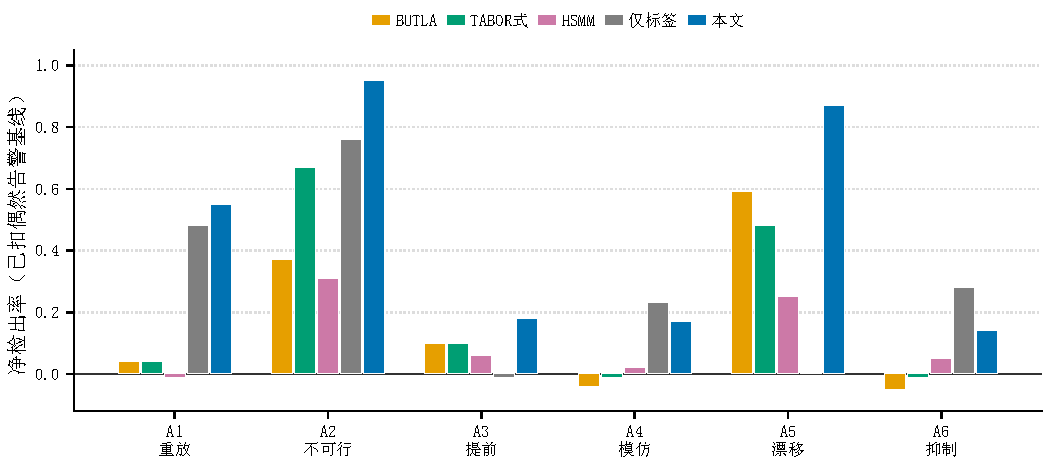
\includegraphics[width=0.98\linewidth]{figures/fig_e1_dr_CN.pdf}
\caption{$\alpha=0.01$、延迟预算 $10$ 条、已扣除偶然告警基线的净检出率。仅标签为马尔可夫消融，而非独立的先行方法。}
\label{fig:e1}
\Description{六类攻击上 BUTLA、TABOR 式、HSMM、仅标签与本文的分组柱状图，本文在 A2 与 A5 最高，仅标签在 A3 与 A5 为零。}
\end{figure}

\begin{figure}[!t]
\centering
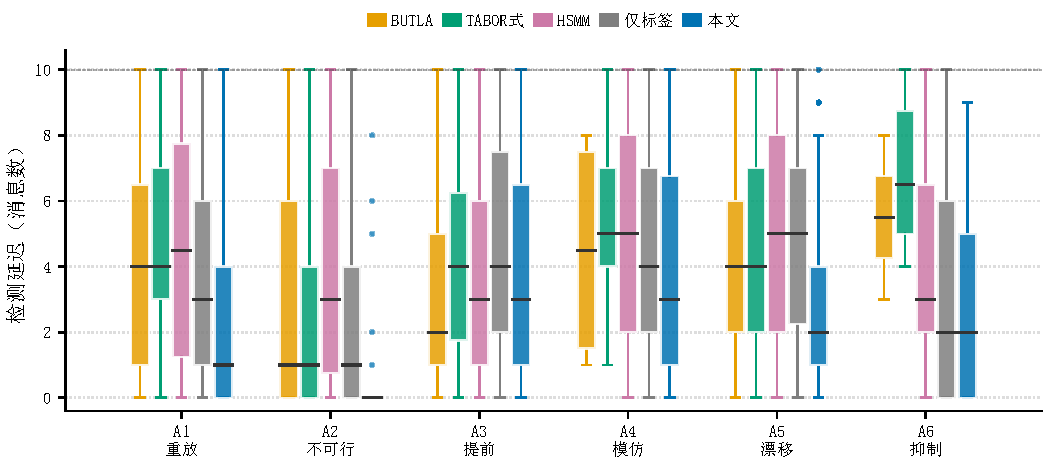
\includegraphics[width=0.98\linewidth]{figures/fig_e1_delay_CN.pdf}
\caption{$\alpha=0.01$、延迟预算 $10$ 条下，各方法在六类攻击上的检测延迟（消息数）。箱线仅含预算内检出；未检出见净检出率。}
\label{fig:e1delay}
\Description{六类攻击上 BUTLA、TABOR 式、HSMM、仅标签与本文的分组箱线图，纵轴为检测延迟消息数。}
\end{figure}

\begin{table}[!t]
\renewcommand{\arraystretch}{1.12}
\caption{测试折纯良性流（$508$ 条事件）上的告警间隔。三个种子共用同一条良性流，告警次数按该流计；间隔含流起点至首次告警。告警过少，不足以估计 $\mathrm{ARL}_0$。}
\label{tab:arl0}
\centering
\small
\begin{tabular}{lccc}
\toprule
方法 & 中位间隔 & 均值间隔 & 告警次数 \\
\midrule
{B1} {BUTLA} & $21$ & $152$ & $3$ \\
{B2} {TABOR} 式 & $59$ & $158$ & $3$ \\
{B3} {HSMM} & $119$ & $115$ & $4$ \\
仅标签 & $56$ & $83$ & $4$ \\
本文 & $218$ & $218$ & $2$ \\
\bottomrule
\end{tabular}
\end{table}

\begin{figure}[!t]
\centering
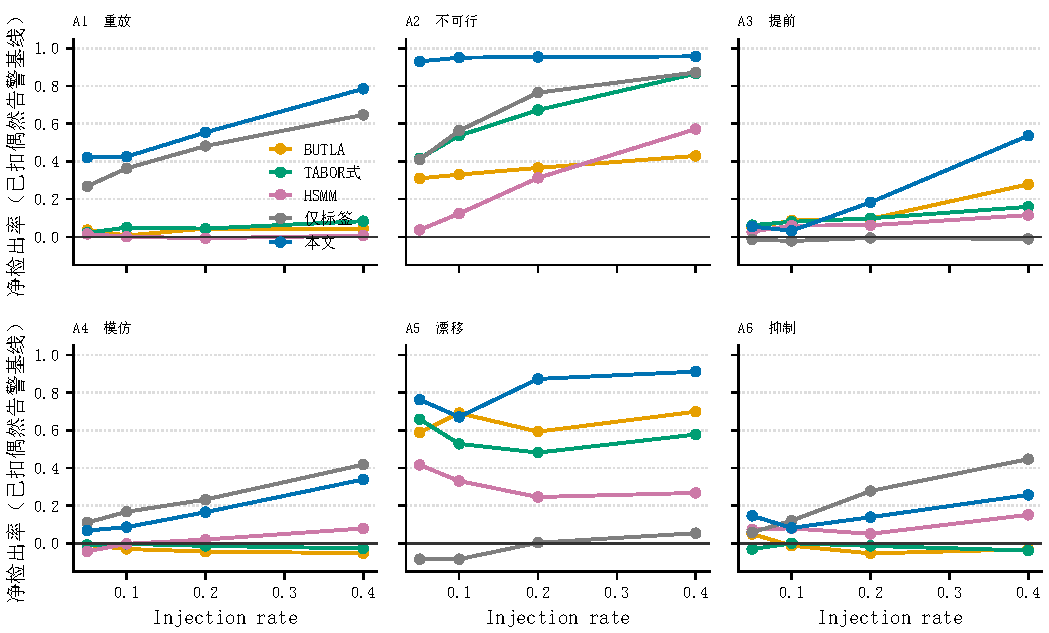
\includegraphics[width=0.98\linewidth]{figures/fig_e1_rate_CN.pdf}
\caption{净检出率随注入率（$5\%$--$40\%$）的变化。按攻击族分设子图，可据此判断结论是否随攻击密度升高而失效。}
\label{fig:e1rate}
\Description{六个攻击族子图，横轴注入率，纵轴净检出率，五条方法曲线。}
\end{figure}

\subsection{消融}
\label{sec:e2}

消融实验沿用主表的判决流程与 $\alpha=0.01$，并\emph{固定每路误报预算}，以避免``去掉一路通道等同于为其余通道增加预算''的混淆。完整配置在六个攻击族上的均值为 $0.48$。去掉时序通道后均值下降 $0.18$，且 {A3}/{A5} 归零（$0.18\to -0.01$，$0.87\to -0.02$）。去掉时序通道后只剩硬约束层与结构通道，二者都只读取标签，因而在纯时长攻击上没有检出，这与表~\ref{tab:e1}中仅标签消融在同两项上的零检出相互印证。去掉硬约束层后均值下降 $0.08$，降幅集中在 {A2}（$0.95\to0.70$）与 {A1}（$0.55\to0.42$）。去掉结构通道后均值下降 $0.05$，降幅集中在 {A6}（$0.14\to-0.02$）与 {A4}（$0.17\to0.08$）。$\alpha=0.05$ 下三项降幅依次为 $0.16$、$0.04$、$0.03$，次序不变。三路中只有时序通道不可替代，它是 {A3}/{A5} 检出的唯一来源。图~\ref{fig:e2}给出按攻击族的对照与均值变化。

\begin{figure}[!t]
\centering
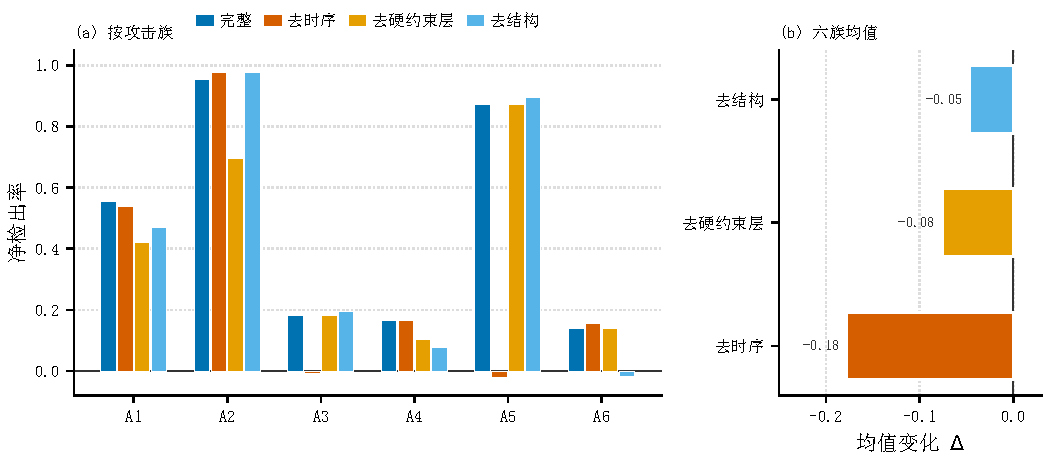
\includegraphics[width=0.98\linewidth]{figures/fig_e2_ablation_CN.pdf}
\caption{生产三路的消融（$\alpha=0.01$，每路误报预算固定，三个注入种子均值，已扣除偶然告警基线）。去掉时序后 {A3}/{A5} 归零；去掉硬约束层的降幅集中在 {A2}/{A1}，去掉结构的降幅集中在 {A6}/{A4}。}
\label{fig:e2}
\Description{左图为完整、去时序、去硬约束层、去结构在六类攻击上的柱状对照；右图为均值下降 0.18、0.08、0.05。}
\end{figure}

共形校准的作用体现在误报一侧：在第~\ref{sec:e4}~节的分层校准集上，单侧阈值改用高斯分位后，测试集经验误报由 $0.0126$ 升至 $0.0168$（名义 $0.01$）。

方法中的几项设计选择也由实测决定。时序通道若输入截断后的参数化 $p$ 值而非 $-z$，{A3} 的单消息检出由 $0.43$ 降至 $0.06$（与表~\ref{tab:coverage}同一口径）。物料令牌守恒约束曾作为候选通道，但其良性违反率过高、端到端净贡献为零（第~\ref{sec:limitations}~节），因此未纳入生产配置，也不占用误报预算。

\subsection{相对提前量扫描}
\label{sec:e4}

在真实停留时长上施加注入 $\tau\mapsto(1-\rho)\tau$。命题~\ref{prop:rho}中的 $\rho^*$ 采用全局拟合折的 $\sigma=0.236$（不对协变量作条件化），$\alpha=0.01$ 单侧时 $\rho^*=42.2\%$。表~\ref{tab:e4}与图~\ref{fig:e4}中的理论值是按工序分组后的混合预测（第~\ref{sec:bound}~节），与实测值在全区间的平均绝对偏差为 $0.027$（校准折与测试折分别自助重抽 $2000$ 次，$95\%$ 区间 $[0.018,0.035]$；$20$ 个折划分种子下为 $0.012$--$0.031$）。$\rho=0.30<\rho^*$ 时实测单消息检出已达 $0.52$，$\rho=0.40\approx\rho^*$ 时为 $0.74$，而单一高斯分布在 $\rho^*$ 处的检出仅为 $1/2$，这正是混合功效曲线所预测的现象。

{CUSUM} 能把弱信号转化为可用的检测能力：该实验在分层校准集上以参数化左尾 $p$ 值驱动 {CUSUM}，门限对应 $\mathrm{ARL}_0=500$，延迟预算 $40$ 条。$\rho=0.15$ 时单消息检出为 $0.21$，累积后升至 $0.55$，中位延迟 $15$ 条；$\rho=0.20$ 时升至 $0.85$；$\rho=0.30$ 时为 $0.93$，中位延迟 $7$ 条，见图~\ref{fig:delay}。检出率在约 $0.96$ 处饱和，未检出部分来自 $\sigma$ 极大的分组，与``整体可检测性由变异最大的工序决定''一致。

\begin{table}[!t]
\renewcommand{\arraystretch}{1.12}
\caption{$\alpha=0.01$ 单侧下的相对提前量扫描（分层校准集 $n_{\mathrm{cal}}=701$、测试 $715$ 条）。位移 $\Delta=\log(1-\rho)$；$\bar\sigma$ 为测试分组的平均时序变异（约 $0.24$）；理论列为按工序混合后的预测。}
\label{tab:e4}
\centering
\small
\begin{tabular}{ccccc}
\toprule
$\rho$ & $\lvert\Delta\rvert$ & $\lvert\Delta\rvert/\bar\sigma$ & 实测 {DR} & 理论 \\
\midrule
$0.05$ & $0.051$ & $0.21$ & $0.062$ & $0.057$ \\
$0.10$ & $0.105$ & $0.44$ & $0.073$ & $0.132$ \\
$0.15$ & $0.163$ & $0.68$ & $0.206$ & $0.239$ \\
$0.20$ & $0.223$ & $0.93$ & $0.291$ & $0.338$ \\
$0.30$ & $0.357$ & $1.49$ & $0.516$ & $0.537$ \\
$0.40$ & $0.511$ & $2.13$ & $0.740$ & $0.745$ \\
$0.50$ & $0.693$ & $2.89$ & $0.899$ & $0.878$ \\
\bottomrule
\end{tabular}
\end{table}

\begin{figure}[!t]
\centering
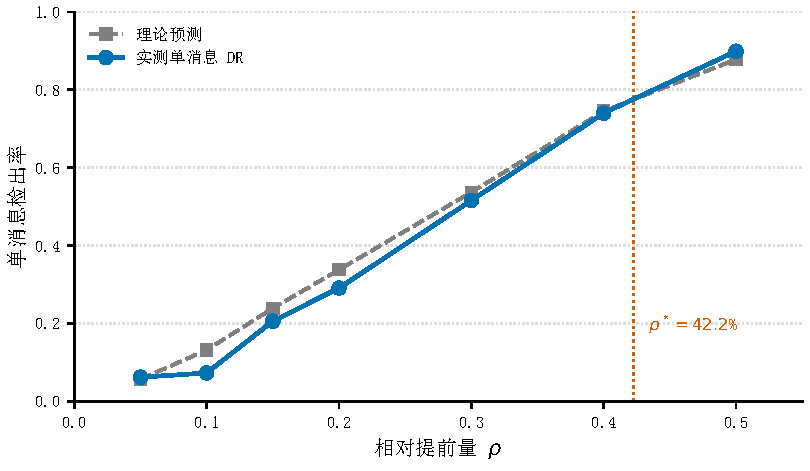
\includegraphics[width=0.82\linewidth]{figures/fig_e4_rho_CN.pdf}
\caption{单消息检出率随相对提前量的变化。理论列为分组混合预测；竖线为全局 $\sigma=0.236$ 下的 $\rho^*=42.2\%$。}
\label{fig:e4}
\Description{实测单消息检出率与按工序混合的理论预测随相对提前量上升；竖线标出全局 sigma 下的 rho 星，该处混合功效已明显高于二分之一。}
\end{figure}

\begin{figure}[!t]
\centering
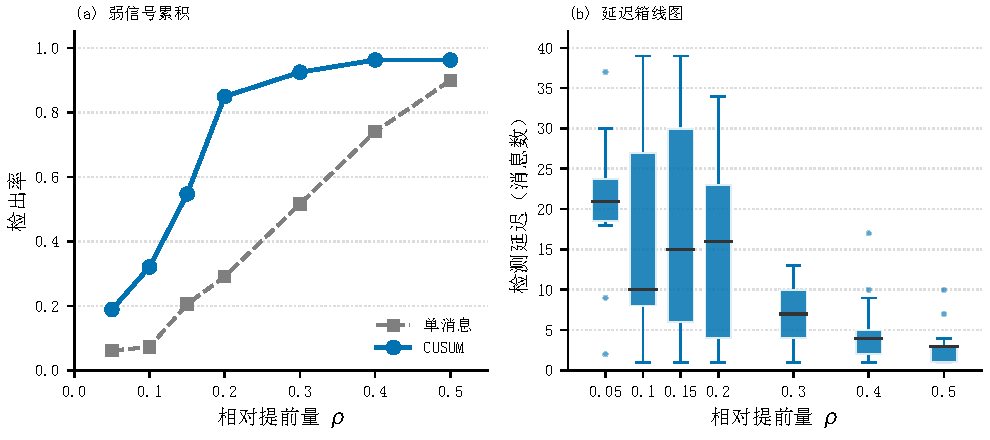
\includegraphics[width=0.98\linewidth]{figures/fig_delay_CN.pdf}
\caption{{CUSUM} 相对单消息阈值的功效，以及检测延迟箱线图。分层校准集上以参数化左尾 $p$ 值驱动，门限对应 $\mathrm{ARL}_0=500$，延迟预算 $40$ 条，$53$ 条测试子流。箱线只含预算内检出的注入；未检出为删失，见主表净检出率。}
\label{fig:delay}
\Description{左图 CUSUM 检出率在小相对提前量下明显高于单消息；右图中位延迟随相对提前量下降。}
\end{figure}

\subsection{部署条件与适用边界}
\label{sec:boundary}
\label{sec:e5}
\label{sec:robust}
\label{sec:gate}
\label{sec:e6}
\label{sec:e8}

前述各节给出主结果。本节报告部署前必须说明的四组数据。

第一，时间序划分下的误报。共形保证依赖可交换性，而实际部署只能按时间先后划分数据。表~\ref{tab:fprsplit}按作业实例以 $75\%/25\%$ 切分拟合与测试（测试集约 $636$ 条消息）：随机折取 $5$ 次随机切分；时间序折只有一种切分，$5$ 个种子仅改变拟合与共形校准中的随机化，故标准差很小。由该表可见：随机划分下的经验误报贴近名义值；按时间序划分时，$\alpha=0.01$ 下时序通道升至 $0.024$，结构通道升至 $0.012$。随数据发布的 $16$ 个工作流之间，转移集合的 {Jaccard} 相似度中位数仅为 $0.324$，说明不同工作流的转移结构差异很大，因此新产品型号须重新校准，或按型号分层校准。该数值是逐通道的单消息误报，与第~\ref{sec:e1}~节攻击流中的序贯误报 $0.004$ 统计方式不同；若序贯门限也取自校准折，本文方法的序贯误报为 $0.030$（第~\ref{sec:e1}~节），与逐通道结果同向。

第二，日志内部的压力测试（表~\ref{tab:shift}）。官方含错版本的时序误报为 $0.112$，来源是数据采集缺陷造成的良性时序异常，而非攻击；未出现工作流上的时序误报为 $0.067$。硬约束层在这两种情形下的误报分别为 $0.003$ 与 $0$。产品切换属于分布漂移，时序通道须按型号重新校准，硬约束层则无此必要。

第三，时长核的重新标定。将拟合折的 $\sigma$ 人为加倍后，$\rho=0.30$ 时的单消息/{CUSUM} 检出由 $0.52/0.94$ 降至 $0.22/0.45$；$\sigma\approx0.96$ 时单消息检出仅剩 $0.05$，适用边界由变异最大的工序划定。表~\ref{tab:e6}在自建仿真产线上进一步演示时长核必须按场景重新标定。三个场景共享操作词表与可行性掩码 $\mathbf F$：场景~I 含 $2$ 台自动导引车与 $1$ 台机械臂，$\sigma=0.12$，行程较短；场景~II 含 $4$ 台自动导引车与 $2$ 台机械臂，$\sigma=0.12$，行程较长；场景~III 布局同场景~I，$\sigma=0.35$。在场景~II 上，使用本场景标定的时长核时 {A3} 检出为 $0.56$，换用场景~I 的时长核后降至 $0.06$（该场景仅 $18$ 条 {A3} 注入，即 $10/18$ 对 $1/18$）；反向迁移（II$\to$I）则使时序误报达到 $0.493$。所有设置下硬约束层的误报均为 $0$，原因是各场景的 $\mathbf F$ 相同。

第四，门控与计算开销。在持续 $200$ 条、$\rho=0.30$ 的提前上报下，关闭门控会将 $26.4\%$ 的伪造提前量引入基线（$200/200$ 次更新全部生效），启用门控后降至 $1.4\%$（$3/200$）。单核逐事件处理时延的中位数为 $123\,\mu\mathrm{s}$（$p_{95}=191\,\mu\mathrm{s}$，$n=1{,}524$）；复制设备名以扩大规模后，中位时延不随规模上升。本文未在专用控制器上实测。

\begin{table}[!t]
\renewcommand{\arraystretch}{1.12}
\caption{逐通道共形经验误报。按作业实例 $75\%/25\%$ 切分（测试集约 $636$ 条消息）；随机折为 $5$ 次随机切分，时间序折为同一切分下 $5$ 个种子，均值$\pm$标准差。}
\label{tab:fprsplit}
\centering
\small
\begin{tabular}{lcccc}
\toprule
通道 & \multicolumn{2}{c}{随机折} & \multicolumn{2}{c}{时间序} \\
\cmidrule(lr){2-3}\cmidrule(lr){4-5}
 & $\alpha{=}0.05$ & $\alpha{=}0.01$ & $\alpha{=}0.05$ & $\alpha{=}0.01$ \\
\midrule
时序 & $0.051{\pm}0.007$ & $0.006{\pm}0.005$ & $0.098{\pm}0.001$ & $0.024{\pm}0.001$ \\
结构 & $0.048{\pm}0.013$ & $0.008{\pm}0.006$ & $0.064{\pm}0.003$ & $0.012{\pm}0.001$ \\
\bottomrule
\end{tabular}
\end{table}

\begin{table}[!t]
\renewcommand{\arraystretch}{1.12}
\caption{同一份 {Trier} 日志内部的压力测试（$\alpha=0.01$，不注入）。含错版本由原作者发布；未出现工作流由时间序测试折切分得到。}
\label{tab:shift}
\label{tab:cprime}
\label{tab:e9}
\centering
\small
\begin{tabular}{lcccc}
\toprule
场景 & $n$ & 硬约束层 & 时序 & 结构 \\
\midrule
清洗时间序测试折 & $508$ & $0.000$ & $0.024$ & $0.012$ \\
官方含错全日志 & $2{,}778$ & $0.003$ & $0.112$ & $0.011$ \\
已出现工作流 & $329$ & $0.000$ & $0.000$ & $0.012$ \\
未出现工作流 & $179$ & $0.000$ & $0.067$ & $0.006$ \\
\bottomrule
\end{tabular}
\end{table}

\begin{table}[!t]
\renewcommand{\arraystretch}{1.12}
\caption{自建仿真场景上时长核的重新标定（$\alpha=0.01$，$\rho=0.30$）。前三列为各通道误报，{A3} 列为时序通道的单消息检出；``I$\to$II''表示在场景~I 上标定、在场景~II 上检测。各场景良性事件 $69$--$90$ 条、{A3} 注入 $13$--$18$ 条。}
\label{tab:e6}
\centering
\small
\begin{tabular}{lcccc}
\toprule
设置 & 硬约束层 & 时序 & 结构 & {A3} \\
\midrule
场景~I & $0.000$ & $0.000$ & $0.014$ & $0.462$ \\
场景~II & $0.000$ & $0.000$ & $0.011$ & $0.556$ \\
场景~III & $0.000$ & $0.000$ & $0.014$ & $0.308$ \\
I$\to$II & $0.000$ & $0.000$ & $0.000$ & $0.056$ \\
I$\to$III & $0.000$ & $0.101$ & $0.000$ & $0.385$ \\
II$\to$I & $0.000$ & $0.493$ & $0.000$ & $0.692$ \\
\bottomrule
\end{tabular}
\end{table}

% ============================================================
%  第 7 章：结论
% ============================================================
\section{结论}
\label{sec:conclusion}

\subsection{结论与贡献}
\label{sec:contributions}

本文形式化了带生命周期的离散活动事件上的注入检测问题。理论上，本文以编号命题（命题~\ref{prop:ta}）表明仅依据标签预测概率设定阈值的检测族，在零误报约束下对标签自洽的注入不提供超出可行性掩码的增量，并给出临界相对提前量 $\rho^*(\alpha,\sigma)$。

方法上，本文以参考模型可行性掩码构成硬约束层（清洗后的正常数据上零违反），以按（设备，操作）分组的分布型停留时长构成时序通道，两路统计通道经共形预测校准后由 {CUSUM} 检验累积。与分解式计时自动机和工段内依赖模型相比，本文的差别有两点：分布型时长使落在守卫之内的提前上报可被累积；可行性来自参考模型，而不是从日志中学习得到。

实验表明，物理不可行注入由可行性掩码覆盖（净检出 $0.95$）；渐变漂移上本文取得 $0.87$，而仅标签消融为零；提前完成重放在注入率 $20\%$ 时为 $0.18$，高于 {BUTLA}，与 {TABOR} 式基线的差异不显著；临界相对提前量模型所预测的混合功效曲线与实测吻合。这些结果说明，对于带生命周期的工业活动事件，参考模型可行性与分布型停留时长是仅依赖标签的检测所缺失的两类证据；{A4}/{A6} 上的劣势则说明，这两类证据不能替代工作流结构。

\subsection{局限}
\label{sec:limitations}

\textbf{(1) 状态模仿与消息抑制缺少专属检测通道。}
在 {A4}/{A6} 上，本文的检出低于仅标签消融。可能原因有二，影响尚未分离：三路分摊后结构通道只获得 $\alpha/3$；结构通道的状态取操作名，对设备不敏感。该局限限定``六类均值''的比较，不影响关于 {A2} 与 {A3}/{A5} 的主张。

\textbf{(2) 物料流不变量在缺少工件身份时无法作为可靠约束。}
良性违反率 $q$ 由训练折的 $0.0054$ 升至部署流的 $0.047$，$\alpha=0.01$ 下单消息检出上限仅为 $0.21$。跨 case 的近似工件身份可将 $q$ 降至 $2.3\%$，仍高于 $\alpha$，端到端性能与不用该约束时持平，因此令牌约束未纳入检测器。该局限不影响本文的三项主张，只说明硬约束层尚不能覆盖跨设备的物料流伪造。

\textbf{(3) 主评测仅使用一份公开日志、合成注入与复现基线。}
主评测仅有一份同时具备 {BPMN} 与活动生命周期的公开日志，攻击由可复现的注入器合成，基线按原文结构约束复现而非使用官方代码，也未与含时间特征的学习型序列模型对照。日志内部的工作流切分、官方含错版本与未出现工作流仅用于压力测试，不能替代第二份外部数据；按时间序划分时共形保证不再自动成立，时长核也不能跨场景直接迁移（第~\ref{sec:boundary}~节）。该局限威胁 {A2} 与 {A3}/{A5} 结果的外部效度，不影响命题~\ref{prop:ta}。

\subsection{未来工作}
\label{sec:future_work}

\textbf{(1) 在带工件标识的产线上验证物料令牌约束。}
对应局限~(2)。具备工件身份后，若部署阶段的良性违反率能降至 $\alpha$ 量级，令牌守恒可作为硬约束层的补充，用于检测跨设备的物料流伪造。

\textbf{(2) 设计不依赖攻击标签的通道间误报预算分配规则。}
对应局限~(1)。现行的 $\alpha/3$ 是并行``或''判决下的 Bonferroni 均分，{A4}/{A6} 上的劣势可能与结构通道仅获得 $\alpha/3$ 有关。分配规则不得利用攻击标签反向调整阈值。

\textbf{(3) 引入第二份外部数据、官方基线实现与学习型序列基线。}
对应局限~(3)。需要另一份同时具备 {BPMN} 与活动生命周期的公开日志，或可对接本日志格式的官方基线实现，并补充含时间特征的学习型序列模型作为对照，以检验结论的外部效度。

\textbf{(4) 研究时长核的在线重标定。}
对应局限~(3) 与第~\ref{sec:boundary}~节。自建场景表明，时长核跨场景迁移会使 {A3} 检出大幅下降或误报升高，而可行性掩码无需重估。后续可研究在门控保护下按产品型号自适应更新时长核，使检测器在产品切换后无需完整重新拟合。

\section{数据可用性}
\label{sec:data}

{Fischertechnik} {Trier} 智能工厂事件日志由原作者发布~\cite{malburg2022trier}，数据副本见 {Figshare} \texttt{10.6084/m9.figshare.20130794}。注入协议、基线复现、诊断脚本与评测存档均在配套代码库中，审稿期间可向通讯作者索取，录用后公开；主表与箱线图均从 JSON 存档读取，不手工填写分位数。论文级 {CSV} 由 \texttt{py -m tools.export\_experiments} 从存档汇总。自建场景~I/II/III（代码中的配置 {A}/{B}/{C}）由 \texttt{algorithm/plant.py} 按种子重新生成。{HAI} 仅用于数据字典核验，未导入 {CSV}。

\begin{acks}
感谢 {University of Trier} 发布带 {BPMN} 参考模型的 {IoT} 事件日志，使可行性掩码得以由外部参考模型提供，而非从日志中学习得到。
\end{acks}

% Bibliography (placed at document end)
\bibliographystyle{ACM-Reference-Format}
\bibliography{reference-base,reference-suggested}

\end{document}